\documentclass[acmtist]{acmtrans2m}
\usepackage{amsfonts, amsmath, amssymb, amsthm}
\usepackage{hyperref, graphicx, verbatim, listings, multirow}
\usepackage{algorithm, algorithmic}
% \usepackage{fancyhdr}

% \ifdefined\makeindex
%   \message{\string\makeindex\space is defined}\usepackage{natbib}\setcitestyle{super}%
% \else
%   \message{no command \string\makeindex}%
% \fi

% To remove excessive vertical spacing while using itemize etc.
\usepackage{enumitem}
\setlist{nolistsep}

% Include and configure tikz
\usepackage{tikz}
\usetikzlibrary{arrows,decorations,fit,backgrounds}

\tikzstyle{gm-var-constant}=[rectangle, draw, fill=black!30, thick, minimum size=1mm]
\tikzstyle{gm-var-hidden}=[circle, draw, thick, minimum size=1mm]
\tikzstyle{gm-var-seen}=[gm-var-hidden, fill=black!30, minimum size=1mm]
\tikzstyle{gm-plate} = [thick,draw=black,rounded corners=2mm]

% For clique trees.
\tikzstyle{ct-shared-nodes}=[rectangle, draw, fill=black!30, thick, minimum size=1mm]
\tikzstyle{ct-clique}=[circle, draw, thick, minimum size=1mm]


% \usepackage[bottom]{footmisc}

% COnfigure the listings package: break lines.
\lstset{breaklines=true}

\setcounter{tocdepth}{3}

% Lets verbatim and verb environments automatically break lines.
\makeatletter
\def\@xobeysp{ }
\makeatother
% \lstset{breaklines=true,basicstyle=\ttfamily}

% Packages not included:
% For multiline comments, use caption package. But this conflicts with hyperref while making html files.
% subfigure conflicts with use with memoir style-sheet.

% Use something like:
% % Use something like:
% % Use something like:
% \input{../../macros}

% groupings of objects.
\newcommand{\set}[1]{\ensuremath{\left\{ #1 \right\}}}
\newcommand{\seq}[1]{\ensuremath{\left(#1\right)}}
\newcommand{\ang}[1]{\ensuremath{\langle#1\rangle}}
\newcommand{\tuple}[1]{\ensuremath{\left(#1\right)}}
\newcommand{\size}[1]{\ensuremath{\left| #1\right|}}

% numerical shortcuts.
\newcommand{\abs}[1]{\ensuremath{\left| #1\right|}}
\newcommand{\floor}[1]{\ensuremath{\left\lfloor #1 \right\rfloor}}
\newcommand{\ceil}[1]{\ensuremath{\left\lceil #1 \right\rceil}}

% linear algebra shortcuts.
\newcommand{\change}{\ensuremath{\Delta}}
\newcommand{\norm}[1]{\ensuremath{\left\| #1\right\|}}
\newcommand{\dprod}[1]{\ensuremath{\langle#1\rangle}}
\newcommand{\linspan}[1]{\ensuremath{\langle#1\rangle}}
\newcommand{\conj}[1]{\ensuremath{\overline{#1}}}
\newcommand{\der}{\ensuremath{\frac{d}{dx}}}
\newcommand{\lap}{\ensuremath{\Delta}}
\newcommand{\kron}{\ensuremath{\otimes}}
\newcommand{\nperp}{\ensuremath{\nvdash}}

\newcommand{\mat}[1]{\left[ \begin{smallmatrix}#1 \end{smallmatrix} \right]}

% derivatives and limits
\newcommand{\partder}[2]{\ensuremath{\frac{\partial #1}{\partial #2}}}
\newcommand{\partdern}[3]{\ensuremath{\frac{\partial^{#3} #1}{\partial #2^{#3}}}}
\newcommand{\gradient}{\ensuremath{\nabla}}
\newcommand{\subdifferential}{\ensuremath{\partial}}

% Arrows
\newcommand{\diverge}{\ensuremath{\nearrow}}
\newcommand{\notto}{\ensuremath{\nrightarrow}}
\newcommand{\up}{\ensuremath{\uparrow}}
\newcommand{\down}{\ensuremath{\downarrow}}
% gets and gives are defined!

% ordering operators
\newcommand{\oleq}{\preceq}
\newcommand{\ogeq}{\succeq}

% programming and logic operators
\newcommand{\dfn}{:=}
\newcommand{\assign}{:=}
\newcommand{\co}{\ co\ }
\newcommand{\en}{\ en\ }


% logic operators
\newcommand{\xor}{\ensuremath{\oplus}}
\newcommand{\Land}{\ensuremath{\bigwedge}}
\newcommand{\Lor}{\ensuremath{\bigvee}}
\newcommand{\finish}{\ensuremath{\Box}}
\newcommand{\contra}{\ensuremath{\Rightarrow \Leftarrow}}
\newcommand{\iseq}{\ensuremath{\stackrel{_?}{=}}}


% Set theory
\newcommand{\symdiff}{\ensuremath{\Delta}}
\newcommand{\union}{\ensuremath{\cup}}
\newcommand{\inters}{\ensuremath{\cap}}
\newcommand{\Union}{\ensuremath{\bigcup}}
\newcommand{\Inters}{\ensuremath{\bigcap}}
\newcommand{\nullSet}{\ensuremath{\phi}}


% graph theory
\newcommand{\nbd}{\Gamma}

% Script alphabets
% For reals, use \Re

% greek letters
\newcommand{\eps}{\ensuremath{\epsilon}}
\newcommand{\del}{\ensuremath{\delta}}
\newcommand{\ga}{\ensuremath{\alpha}}
\newcommand{\gb}{\ensuremath{\beta}}
\newcommand{\gd}{\ensuremath{\del}}
\newcommand{\gp}{\ensuremath{\pi}}
\newcommand{\gf}{\ensuremath{\phi}}
\newcommand{\gh}{\ensuremath{\eta}}
\newcommand{\gF}{\ensuremath{\Phi}}
\newcommand{\gl}{\ensuremath{\lambda}}
\newcommand{\gm}{\ensuremath{\mu}}
\newcommand{\gn}{\ensuremath{\nu}}
\newcommand{\gr}{\ensuremath{\rho}}
\newcommand{\gs}{\ensuremath{\sigma}}
\newcommand{\gt}{\ensuremath{\theta}}
\newcommand{\gx}{\ensuremath{\xi}}

\newcommand{\sw}{\ensuremath{\sigma}}
\newcommand{\SW}{\ensuremath{\Sigma}}
\newcommand{\ew}{\ensuremath{\lambda}}
\newcommand{\EW}{\ensuremath{\Lambda}}

\newcommand{\Del}{\ensuremath{\Delta}}
\newcommand{\gD}{\ensuremath{\Delta}}
\newcommand{\gG}{\ensuremath{\Gamma}}
\newcommand{\gO}{\ensuremath{\Omega}}
\newcommand{\gS}{\ensuremath{\Sigma}}

% Bold english letters.
\newcommand{\bA}{\ensuremath{\mathbf{A}}}
\newcommand{\bB}{\ensuremath{\mathbf{B}}}
\newcommand{\bC}{\ensuremath{\mathbf{C}}}
\newcommand{\bD}{\ensuremath{\mathbf{D}}}
\newcommand{\bE}{\ensuremath{\mathbf{E}}}
\newcommand{\bF}{\ensuremath{\mathbf{F}}}
\newcommand{\bG}{\ensuremath{\mathbf{G}}}
\newcommand{\bH}{\ensuremath{\mathbf{H}}}
\newcommand{\bI}{\ensuremath{\mathbf{I}}}
\newcommand{\bJ}{\ensuremath{\mathbf{J}}}
\newcommand{\bK}{\ensuremath{\mathbf{K}}}
\newcommand{\bL}{\ensuremath{\mathbf{L}}}
\newcommand{\bM}{\ensuremath{\mathbf{M}}}
\newcommand{\bN}{\ensuremath{\mathbf{N}}}
\newcommand{\bO}{\ensuremath{\mathbf{O}}}
\newcommand{\bP}{\ensuremath{\mathbf{P}}}
\newcommand{\bQ}{\ensuremath{\mathbf{Q}}}
\newcommand{\bR}{\ensuremath{\mathbf{R}}} % PROSPER defines \R
\newcommand{\bS}{\ensuremath{\mathbf{S}}}
\newcommand{\bT}{\ensuremath{\mathbf{T}}}
\newcommand{\bU}{\ensuremath{\mathbf{U}}}
\newcommand{\bV}{\ensuremath{\mathbf{V}}}
\newcommand{\bW}{\ensuremath{\mathbf{W}}}
\newcommand{\bX}{\ensuremath{\mathbf{X}}}
\newcommand{\bY}{\ensuremath{\mathbf{Y}}}
\newcommand{\bZ}{\ensuremath{\mathbf{Z}}}
\newcommand{\bba}{\ensuremath{\mathbf{a}}}
\newcommand{\bbb}{\ensuremath{\mathbf{b}}}
\newcommand{\bbc}{\ensuremath{\mathbf{c}}}
\newcommand{\bbd}{\ensuremath{\mathbf{d}}}
\newcommand{\bbe}{\ensuremath{\mathbf{e}}}
\newcommand{\bbf}{\ensuremath{\mathbf{f}}}
\newcommand{\bbg}{\ensuremath{\mathbf{g}}}
\newcommand{\bbh}{\ensuremath{\mathbf{h}}}
\newcommand{\bbk}{\ensuremath{\mathbf{k}}}
\newcommand{\bbl}{\ensuremath{\mathbf{l}}}
\newcommand{\bbm}{\ensuremath{\mathbf{m}}}
\newcommand{\bbn}{\ensuremath{\mathbf{n}}}
\newcommand{\bbp}{\ensuremath{\mathbf{p}}}
\newcommand{\bbq}{\ensuremath{\mathbf{q}}}
\newcommand{\bbr}{\ensuremath{\mathbf{r}}}
\newcommand{\bbs}{\ensuremath{\mathbf{s}}}  % TIPA defines \s and LaTeX \ss!
\newcommand{\bbt}{\ensuremath{\mathbf{t}}}
\newcommand{\bbu}{\ensuremath{\mathbf{u}}}
\newcommand{\bbv}{\ensuremath{\mathbf{v}}}
\newcommand{\bbw}{\ensuremath{\mathbf{w}}}
\newcommand{\bbx}{\ensuremath{\mathbf{x}}}
\newcommand{\bby}{\ensuremath{\mathbf{y}}}
\newcommand{\bbz}{\ensuremath{\mathbf{z}}}
\newcommand{\0}{\ensuremath{\mathbf{0}}}
\newcommand{\1}{\ensuremath{\mathbf{1}}}


% Formatting shortcuts
\newcommand{\red}[1]{\textcolor{red}{#1}}
\newcommand{\green}[1]{\textcolor{green}{#1}}
\newcommand{\magenta}[1]{\textcolor{magenta}{#1}}
\newcommand{\orange}[1]{\textcolor{orange}{#1}}
\newcommand{\gray}[1]{\textcolor{gray}{#1}}
\newcommand{\blue}[1]{\textcolor{blue}{#1}}
\newcommand{\htext}[2]{\texorpdfstring{#1}{#2}}

% Statistics
\newcommand{\distr}{\ensuremath{\sim}}
\newcommand{\stddev}{\ensuremath{\sigma}}
\newcommand{\covmatrix}{\ensuremath{\Sigma}}
\newcommand{\mean}{\ensuremath{\mu}}
\newcommand{\param}{\ensuremath{\gt}}
\newcommand{\ftr}{\ensuremath{\phi}}

% General utility
\newcommand{\todo}[1]{\textbf{[TODO]}] \footnote{TODO: #1}}
\newcommand{\exclaim}[1]{{\textbf{\textit{#1}}}}
\newcommand{\tbc}{[\textbf{Incomplete}]}
\newcommand{\chk}{[\textbf{Check}]}
\newcommand{\oprob}{[\textbf{OP}]:}
\newcommand{\core}[1]{\textbf{Core Idea:}}
\newcommand{\why}{[\textbf{Find proof}]}
\newcommand{\opt}[1]{\textit{#1}}


\renewcommand{\~}{\htext{$\sim$}{~}}

\DeclareMathOperator*{\argmin}{arg\,min}
\DeclareMathOperator*{\argmax}{arg\,max}

% Items pertaining to the headed list.
\newcommand{\headeditem}[1]{\item\textbf{#1}}
\newcommand{\headedsubitem}[1]{\subitem\textbf{#1}}



% groupings of objects.
\newcommand{\set}[1]{\ensuremath{\left\{ #1 \right\}}}
\newcommand{\seq}[1]{\ensuremath{\left(#1\right)}}
\newcommand{\ang}[1]{\ensuremath{\langle#1\rangle}}
\newcommand{\tuple}[1]{\ensuremath{\left(#1\right)}}
\newcommand{\size}[1]{\ensuremath{\left| #1\right|}}

% numerical shortcuts.
\newcommand{\abs}[1]{\ensuremath{\left| #1\right|}}
\newcommand{\floor}[1]{\ensuremath{\left\lfloor #1 \right\rfloor}}
\newcommand{\ceil}[1]{\ensuremath{\left\lceil #1 \right\rceil}}

% linear algebra shortcuts.
\newcommand{\change}{\ensuremath{\Delta}}
\newcommand{\norm}[1]{\ensuremath{\left\| #1\right\|}}
\newcommand{\dprod}[1]{\ensuremath{\langle#1\rangle}}
\newcommand{\linspan}[1]{\ensuremath{\langle#1\rangle}}
\newcommand{\conj}[1]{\ensuremath{\overline{#1}}}
\newcommand{\der}{\ensuremath{\frac{d}{dx}}}
\newcommand{\lap}{\ensuremath{\Delta}}
\newcommand{\kron}{\ensuremath{\otimes}}
\newcommand{\nperp}{\ensuremath{\nvdash}}

\newcommand{\mat}[1]{\left[ \begin{smallmatrix}#1 \end{smallmatrix} \right]}

% derivatives and limits
\newcommand{\partder}[2]{\ensuremath{\frac{\partial #1}{\partial #2}}}
\newcommand{\partdern}[3]{\ensuremath{\frac{\partial^{#3} #1}{\partial #2^{#3}}}}
\newcommand{\gradient}{\ensuremath{\nabla}}
\newcommand{\subdifferential}{\ensuremath{\partial}}

% Arrows
\newcommand{\diverge}{\ensuremath{\nearrow}}
\newcommand{\notto}{\ensuremath{\nrightarrow}}
\newcommand{\up}{\ensuremath{\uparrow}}
\newcommand{\down}{\ensuremath{\downarrow}}
% gets and gives are defined!

% ordering operators
\newcommand{\oleq}{\preceq}
\newcommand{\ogeq}{\succeq}

% programming and logic operators
\newcommand{\dfn}{:=}
\newcommand{\assign}{:=}
\newcommand{\co}{\ co\ }
\newcommand{\en}{\ en\ }


% logic operators
\newcommand{\xor}{\ensuremath{\oplus}}
\newcommand{\Land}{\ensuremath{\bigwedge}}
\newcommand{\Lor}{\ensuremath{\bigvee}}
\newcommand{\finish}{\ensuremath{\Box}}
\newcommand{\contra}{\ensuremath{\Rightarrow \Leftarrow}}
\newcommand{\iseq}{\ensuremath{\stackrel{_?}{=}}}


% Set theory
\newcommand{\symdiff}{\ensuremath{\Delta}}
\newcommand{\union}{\ensuremath{\cup}}
\newcommand{\inters}{\ensuremath{\cap}}
\newcommand{\Union}{\ensuremath{\bigcup}}
\newcommand{\Inters}{\ensuremath{\bigcap}}
\newcommand{\nullSet}{\ensuremath{\phi}}


% graph theory
\newcommand{\nbd}{\Gamma}

% Script alphabets
% For reals, use \Re

% greek letters
\newcommand{\eps}{\ensuremath{\epsilon}}
\newcommand{\del}{\ensuremath{\delta}}
\newcommand{\ga}{\ensuremath{\alpha}}
\newcommand{\gb}{\ensuremath{\beta}}
\newcommand{\gd}{\ensuremath{\del}}
\newcommand{\gp}{\ensuremath{\pi}}
\newcommand{\gf}{\ensuremath{\phi}}
\newcommand{\gh}{\ensuremath{\eta}}
\newcommand{\gF}{\ensuremath{\Phi}}
\newcommand{\gl}{\ensuremath{\lambda}}
\newcommand{\gm}{\ensuremath{\mu}}
\newcommand{\gn}{\ensuremath{\nu}}
\newcommand{\gr}{\ensuremath{\rho}}
\newcommand{\gs}{\ensuremath{\sigma}}
\newcommand{\gt}{\ensuremath{\theta}}
\newcommand{\gx}{\ensuremath{\xi}}

\newcommand{\sw}{\ensuremath{\sigma}}
\newcommand{\SW}{\ensuremath{\Sigma}}
\newcommand{\ew}{\ensuremath{\lambda}}
\newcommand{\EW}{\ensuremath{\Lambda}}

\newcommand{\Del}{\ensuremath{\Delta}}
\newcommand{\gD}{\ensuremath{\Delta}}
\newcommand{\gG}{\ensuremath{\Gamma}}
\newcommand{\gO}{\ensuremath{\Omega}}
\newcommand{\gS}{\ensuremath{\Sigma}}

% Bold english letters.
\newcommand{\bA}{\ensuremath{\mathbf{A}}}
\newcommand{\bB}{\ensuremath{\mathbf{B}}}
\newcommand{\bC}{\ensuremath{\mathbf{C}}}
\newcommand{\bD}{\ensuremath{\mathbf{D}}}
\newcommand{\bE}{\ensuremath{\mathbf{E}}}
\newcommand{\bF}{\ensuremath{\mathbf{F}}}
\newcommand{\bG}{\ensuremath{\mathbf{G}}}
\newcommand{\bH}{\ensuremath{\mathbf{H}}}
\newcommand{\bI}{\ensuremath{\mathbf{I}}}
\newcommand{\bJ}{\ensuremath{\mathbf{J}}}
\newcommand{\bK}{\ensuremath{\mathbf{K}}}
\newcommand{\bL}{\ensuremath{\mathbf{L}}}
\newcommand{\bM}{\ensuremath{\mathbf{M}}}
\newcommand{\bN}{\ensuremath{\mathbf{N}}}
\newcommand{\bO}{\ensuremath{\mathbf{O}}}
\newcommand{\bP}{\ensuremath{\mathbf{P}}}
\newcommand{\bQ}{\ensuremath{\mathbf{Q}}}
\newcommand{\bR}{\ensuremath{\mathbf{R}}} % PROSPER defines \R
\newcommand{\bS}{\ensuremath{\mathbf{S}}}
\newcommand{\bT}{\ensuremath{\mathbf{T}}}
\newcommand{\bU}{\ensuremath{\mathbf{U}}}
\newcommand{\bV}{\ensuremath{\mathbf{V}}}
\newcommand{\bW}{\ensuremath{\mathbf{W}}}
\newcommand{\bX}{\ensuremath{\mathbf{X}}}
\newcommand{\bY}{\ensuremath{\mathbf{Y}}}
\newcommand{\bZ}{\ensuremath{\mathbf{Z}}}
\newcommand{\bba}{\ensuremath{\mathbf{a}}}
\newcommand{\bbb}{\ensuremath{\mathbf{b}}}
\newcommand{\bbc}{\ensuremath{\mathbf{c}}}
\newcommand{\bbd}{\ensuremath{\mathbf{d}}}
\newcommand{\bbe}{\ensuremath{\mathbf{e}}}
\newcommand{\bbf}{\ensuremath{\mathbf{f}}}
\newcommand{\bbg}{\ensuremath{\mathbf{g}}}
\newcommand{\bbh}{\ensuremath{\mathbf{h}}}
\newcommand{\bbk}{\ensuremath{\mathbf{k}}}
\newcommand{\bbl}{\ensuremath{\mathbf{l}}}
\newcommand{\bbm}{\ensuremath{\mathbf{m}}}
\newcommand{\bbn}{\ensuremath{\mathbf{n}}}
\newcommand{\bbp}{\ensuremath{\mathbf{p}}}
\newcommand{\bbq}{\ensuremath{\mathbf{q}}}
\newcommand{\bbr}{\ensuremath{\mathbf{r}}}
\newcommand{\bbs}{\ensuremath{\mathbf{s}}}  % TIPA defines \s and LaTeX \ss!
\newcommand{\bbt}{\ensuremath{\mathbf{t}}}
\newcommand{\bbu}{\ensuremath{\mathbf{u}}}
\newcommand{\bbv}{\ensuremath{\mathbf{v}}}
\newcommand{\bbw}{\ensuremath{\mathbf{w}}}
\newcommand{\bbx}{\ensuremath{\mathbf{x}}}
\newcommand{\bby}{\ensuremath{\mathbf{y}}}
\newcommand{\bbz}{\ensuremath{\mathbf{z}}}
\newcommand{\0}{\ensuremath{\mathbf{0}}}
\newcommand{\1}{\ensuremath{\mathbf{1}}}


% Formatting shortcuts
\newcommand{\red}[1]{\textcolor{red}{#1}}
\newcommand{\green}[1]{\textcolor{green}{#1}}
\newcommand{\magenta}[1]{\textcolor{magenta}{#1}}
\newcommand{\orange}[1]{\textcolor{orange}{#1}}
\newcommand{\gray}[1]{\textcolor{gray}{#1}}
\newcommand{\blue}[1]{\textcolor{blue}{#1}}
\newcommand{\htext}[2]{\texorpdfstring{#1}{#2}}

% Statistics
\newcommand{\distr}{\ensuremath{\sim}}
\newcommand{\stddev}{\ensuremath{\sigma}}
\newcommand{\covmatrix}{\ensuremath{\Sigma}}
\newcommand{\mean}{\ensuremath{\mu}}
\newcommand{\param}{\ensuremath{\gt}}
\newcommand{\ftr}{\ensuremath{\phi}}

% General utility
\newcommand{\todo}[1]{\textbf{[TODO]}] \footnote{TODO: #1}}
\newcommand{\exclaim}[1]{{\textbf{\textit{#1}}}}
\newcommand{\tbc}{[\textbf{Incomplete}]}
\newcommand{\chk}{[\textbf{Check}]}
\newcommand{\oprob}{[\textbf{OP}]:}
\newcommand{\core}[1]{\textbf{Core Idea:}}
\newcommand{\why}{[\textbf{Find proof}]}
\newcommand{\opt}[1]{\textit{#1}}


\renewcommand{\~}{\htext{$\sim$}{~}}

\DeclareMathOperator*{\argmin}{arg\,min}
\DeclareMathOperator*{\argmax}{arg\,max}

% Items pertaining to the headed list.
\newcommand{\headeditem}[1]{\item\textbf{#1}}
\newcommand{\headedsubitem}[1]{\subitem\textbf{#1}}



% groupings of objects.
\newcommand{\set}[1]{\ensuremath{\left\{ #1 \right\}}}
\newcommand{\seq}[1]{\ensuremath{\left(#1\right)}}
\newcommand{\ang}[1]{\ensuremath{\langle#1\rangle}}
\newcommand{\tuple}[1]{\ensuremath{\left(#1\right)}}
\newcommand{\size}[1]{\ensuremath{\left| #1\right|}}

% numerical shortcuts.
\newcommand{\abs}[1]{\ensuremath{\left| #1\right|}}
\newcommand{\floor}[1]{\ensuremath{\left\lfloor #1 \right\rfloor}}
\newcommand{\ceil}[1]{\ensuremath{\left\lceil #1 \right\rceil}}

% linear algebra shortcuts.
\newcommand{\change}{\ensuremath{\Delta}}
\newcommand{\norm}[1]{\ensuremath{\left\| #1\right\|}}
\newcommand{\dprod}[1]{\ensuremath{\langle#1\rangle}}
\newcommand{\linspan}[1]{\ensuremath{\langle#1\rangle}}
\newcommand{\conj}[1]{\ensuremath{\overline{#1}}}
\newcommand{\der}{\ensuremath{\frac{d}{dx}}}
\newcommand{\lap}{\ensuremath{\Delta}}
\newcommand{\kron}{\ensuremath{\otimes}}
\newcommand{\nperp}{\ensuremath{\nvdash}}

\newcommand{\mat}[1]{\left[ \begin{smallmatrix}#1 \end{smallmatrix} \right]}

% derivatives and limits
\newcommand{\partder}[2]{\ensuremath{\frac{\partial #1}{\partial #2}}}
\newcommand{\partdern}[3]{\ensuremath{\frac{\partial^{#3} #1}{\partial #2^{#3}}}}
\newcommand{\gradient}{\ensuremath{\nabla}}
\newcommand{\subdifferential}{\ensuremath{\partial}}

% Arrows
\newcommand{\diverge}{\ensuremath{\nearrow}}
\newcommand{\notto}{\ensuremath{\nrightarrow}}
\newcommand{\up}{\ensuremath{\uparrow}}
\newcommand{\down}{\ensuremath{\downarrow}}
% gets and gives are defined!

% ordering operators
\newcommand{\oleq}{\preceq}
\newcommand{\ogeq}{\succeq}

% programming and logic operators
\newcommand{\dfn}{:=}
\newcommand{\assign}{:=}
\newcommand{\co}{\ co\ }
\newcommand{\en}{\ en\ }


% logic operators
\newcommand{\xor}{\ensuremath{\oplus}}
\newcommand{\Land}{\ensuremath{\bigwedge}}
\newcommand{\Lor}{\ensuremath{\bigvee}}
\newcommand{\finish}{\ensuremath{\Box}}
\newcommand{\contra}{\ensuremath{\Rightarrow \Leftarrow}}
\newcommand{\iseq}{\ensuremath{\stackrel{_?}{=}}}


% Set theory
\newcommand{\symdiff}{\ensuremath{\Delta}}
\newcommand{\union}{\ensuremath{\cup}}
\newcommand{\inters}{\ensuremath{\cap}}
\newcommand{\Union}{\ensuremath{\bigcup}}
\newcommand{\Inters}{\ensuremath{\bigcap}}
\newcommand{\nullSet}{\ensuremath{\phi}}


% graph theory
\newcommand{\nbd}{\Gamma}

% Script alphabets
% For reals, use \Re

% greek letters
\newcommand{\eps}{\ensuremath{\epsilon}}
\newcommand{\del}{\ensuremath{\delta}}
\newcommand{\ga}{\ensuremath{\alpha}}
\newcommand{\gb}{\ensuremath{\beta}}
\newcommand{\gd}{\ensuremath{\del}}
\newcommand{\gp}{\ensuremath{\pi}}
\newcommand{\gf}{\ensuremath{\phi}}
\newcommand{\gh}{\ensuremath{\eta}}
\newcommand{\gF}{\ensuremath{\Phi}}
\newcommand{\gl}{\ensuremath{\lambda}}
\newcommand{\gm}{\ensuremath{\mu}}
\newcommand{\gn}{\ensuremath{\nu}}
\newcommand{\gr}{\ensuremath{\rho}}
\newcommand{\gs}{\ensuremath{\sigma}}
\newcommand{\gt}{\ensuremath{\theta}}
\newcommand{\gx}{\ensuremath{\xi}}

\newcommand{\sw}{\ensuremath{\sigma}}
\newcommand{\SW}{\ensuremath{\Sigma}}
\newcommand{\ew}{\ensuremath{\lambda}}
\newcommand{\EW}{\ensuremath{\Lambda}}

\newcommand{\Del}{\ensuremath{\Delta}}
\newcommand{\gD}{\ensuremath{\Delta}}
\newcommand{\gG}{\ensuremath{\Gamma}}
\newcommand{\gO}{\ensuremath{\Omega}}
\newcommand{\gS}{\ensuremath{\Sigma}}

% Bold english letters.
\newcommand{\bA}{\ensuremath{\mathbf{A}}}
\newcommand{\bB}{\ensuremath{\mathbf{B}}}
\newcommand{\bC}{\ensuremath{\mathbf{C}}}
\newcommand{\bD}{\ensuremath{\mathbf{D}}}
\newcommand{\bE}{\ensuremath{\mathbf{E}}}
\newcommand{\bF}{\ensuremath{\mathbf{F}}}
\newcommand{\bG}{\ensuremath{\mathbf{G}}}
\newcommand{\bH}{\ensuremath{\mathbf{H}}}
\newcommand{\bI}{\ensuremath{\mathbf{I}}}
\newcommand{\bJ}{\ensuremath{\mathbf{J}}}
\newcommand{\bK}{\ensuremath{\mathbf{K}}}
\newcommand{\bL}{\ensuremath{\mathbf{L}}}
\newcommand{\bM}{\ensuremath{\mathbf{M}}}
\newcommand{\bN}{\ensuremath{\mathbf{N}}}
\newcommand{\bO}{\ensuremath{\mathbf{O}}}
\newcommand{\bP}{\ensuremath{\mathbf{P}}}
\newcommand{\bQ}{\ensuremath{\mathbf{Q}}}
\newcommand{\bR}{\ensuremath{\mathbf{R}}} % PROSPER defines \R
\newcommand{\bS}{\ensuremath{\mathbf{S}}}
\newcommand{\bT}{\ensuremath{\mathbf{T}}}
\newcommand{\bU}{\ensuremath{\mathbf{U}}}
\newcommand{\bV}{\ensuremath{\mathbf{V}}}
\newcommand{\bW}{\ensuremath{\mathbf{W}}}
\newcommand{\bX}{\ensuremath{\mathbf{X}}}
\newcommand{\bY}{\ensuremath{\mathbf{Y}}}
\newcommand{\bZ}{\ensuremath{\mathbf{Z}}}
\newcommand{\bba}{\ensuremath{\mathbf{a}}}
\newcommand{\bbb}{\ensuremath{\mathbf{b}}}
\newcommand{\bbc}{\ensuremath{\mathbf{c}}}
\newcommand{\bbd}{\ensuremath{\mathbf{d}}}
\newcommand{\bbe}{\ensuremath{\mathbf{e}}}
\newcommand{\bbf}{\ensuremath{\mathbf{f}}}
\newcommand{\bbg}{\ensuremath{\mathbf{g}}}
\newcommand{\bbh}{\ensuremath{\mathbf{h}}}
\newcommand{\bbk}{\ensuremath{\mathbf{k}}}
\newcommand{\bbl}{\ensuremath{\mathbf{l}}}
\newcommand{\bbm}{\ensuremath{\mathbf{m}}}
\newcommand{\bbn}{\ensuremath{\mathbf{n}}}
\newcommand{\bbp}{\ensuremath{\mathbf{p}}}
\newcommand{\bbq}{\ensuremath{\mathbf{q}}}
\newcommand{\bbr}{\ensuremath{\mathbf{r}}}
\newcommand{\bbs}{\ensuremath{\mathbf{s}}}  % TIPA defines \s and LaTeX \ss!
\newcommand{\bbt}{\ensuremath{\mathbf{t}}}
\newcommand{\bbu}{\ensuremath{\mathbf{u}}}
\newcommand{\bbv}{\ensuremath{\mathbf{v}}}
\newcommand{\bbw}{\ensuremath{\mathbf{w}}}
\newcommand{\bbx}{\ensuremath{\mathbf{x}}}
\newcommand{\bby}{\ensuremath{\mathbf{y}}}
\newcommand{\bbz}{\ensuremath{\mathbf{z}}}
\newcommand{\0}{\ensuremath{\mathbf{0}}}
\newcommand{\1}{\ensuremath{\mathbf{1}}}


% Formatting shortcuts
\newcommand{\red}[1]{\textcolor{red}{#1}}
\newcommand{\green}[1]{\textcolor{green}{#1}}
\newcommand{\magenta}[1]{\textcolor{magenta}{#1}}
\newcommand{\orange}[1]{\textcolor{orange}{#1}}
\newcommand{\gray}[1]{\textcolor{gray}{#1}}
\newcommand{\blue}[1]{\textcolor{blue}{#1}}
\newcommand{\htext}[2]{\texorpdfstring{#1}{#2}}

% Statistics
\newcommand{\distr}{\ensuremath{\sim}}
\newcommand{\stddev}{\ensuremath{\sigma}}
\newcommand{\covmatrix}{\ensuremath{\Sigma}}
\newcommand{\mean}{\ensuremath{\mu}}
\newcommand{\param}{\ensuremath{\gt}}
\newcommand{\ftr}{\ensuremath{\phi}}

% General utility
\newcommand{\todo}[1]{\textbf{[TODO]}] \footnote{TODO: #1}}
\newcommand{\exclaim}[1]{{\textbf{\textit{#1}}}}
\newcommand{\tbc}{[\textbf{Incomplete}]}
\newcommand{\chk}{[\textbf{Check}]}
\newcommand{\oprob}{[\textbf{OP}]:}
\newcommand{\core}[1]{\textbf{Core Idea:}}
\newcommand{\why}{[\textbf{Find proof}]}
\newcommand{\opt}[1]{\textit{#1}}


\renewcommand{\~}{\htext{$\sim$}{~}}

\DeclareMathOperator*{\argmin}{arg\,min}
\DeclareMathOperator*{\argmax}{arg\,max}

% Items pertaining to the headed list.
\newcommand{\headeditem}[1]{\item\textbf{#1}}
\newcommand{\headedsubitem}[1]{\subitem\textbf{#1}}


% Miguel A. Carreira-Perpinan's LaTeX macros.
% Time-stamp: <07/02/08 02:40:12 miguel>

% Definitions that require only standard LaTeX2e things

% Letters used for matrices and vectors (boldface), for functions (roman), etc.
\newcommand{\A}{\ensuremath{\mathbf{A}}}
\newcommand{\B}{\ensuremath{\mathbf{B}}}
\newcommand{\C}{\ensuremath{\mathbf{C}}}
\newcommand{\D}{\ensuremath{\mathbf{D}}}
\newcommand{\E}{\ensuremath{\mathbf{E}}}
\newcommand{\F}{\ensuremath{\mathbf{F}}}
\newcommand{\G}{\ensuremath{\mathbf{G}}}
\newcommand{\HH}{\ensuremath{\mathbf{H}}}
\newcommand{\I}{\ensuremath{\mathbf{I}}}
\newcommand{\J}{\ensuremath{\mathbf{J}}}
\newcommand{\K}{\ensuremath{\mathbf{K}}}
\newcommand{\LL}{\ensuremath{\mathbf{L}}}
\newcommand{\M}{\ensuremath{\mathbf{M}}}
\newcommand{\N}{\ensuremath{\mathbf{N}}}
\newcommand{\OO}{\ensuremath{\mathbf{O}}}
\newcommand{\PP}{\ensuremath{\mathbf{P}}}
\newcommand{\Q}{\ensuremath{\mathbf{Q}}}
%\newcommand{\R}{\ensuremath{\mathbf{R}}} % PROSPER defines \R
\newcommand{\RR}{\ensuremath{\mathbf{R}}}
\renewcommand{\SS}{\ensuremath{\mathbf{S}}}
\newcommand{\T}{\ensuremath{\mathbf{T}}}
\newcommand{\U}{\ensuremath{\mathbf{U}}}
\newcommand{\V}{\ensuremath{\mathbf{V}}}
\newcommand{\W}{\ensuremath{\mathbf{W}}}
\newcommand{\X}{\ensuremath{\mathbf{X}}}
\newcommand{\Y}{\ensuremath{\mathbf{Y}}}
\newcommand{\Z}{\ensuremath{\mathbf{Z}}}
\renewcommand{\aa}{\ensuremath{\mathbf{a}}}
\renewcommand{\b}{\ensuremath{\mathbf{b}}}
\renewcommand{\c}{\ensuremath{\mathbf{c}}}
\newcommand{\dd}{\ensuremath{\mathbf{d}}}
\newcommand{\e}{\ensuremath{\mathbf{e}}}
\newcommand{\f}{\ensuremath{\mathbf{f}}}
\newcommand{\g}{\ensuremath{\mathbf{g}}}
\newcommand{\h}{\ensuremath{\mathbf{h}}}
\newcommand{\bk}{\ensuremath{\mathbf{k}}}
\newcommand{\bl}{\ensuremath{\mathbf{l}}}
\newcommand{\m}{\ensuremath{\mathbf{m}}}
\newcommand{\n}{\ensuremath{\mathbf{n}}}
\newcommand{\p}{\ensuremath{\mathbf{p}}}
\newcommand{\q}{\ensuremath{\mathbf{q}}}
\newcommand{\rr}{\ensuremath{\mathbf{r}}}
\newcommand{\sss}{\ensuremath{\mathbf{s}}}  % TIPA defines \s and LaTeX \ss!
\renewcommand{\t}{\ensuremath{\mathbf{t}}}
\newcommand{\uu}{\ensuremath{\mathbf{u}}}
\newcommand{\vv}{\ensuremath{\mathbf{v}}}
%\renewcommand{\v}{\ensuremath{\mathbf{v}}}
\newcommand{\w}{\ensuremath{\mathbf{w}}}
\newcommand{\x}{\ensuremath{\mathbf{x}}}
\newcommand{\y}{\ensuremath{\mathbf{y}}}
\newcommand{\z}{\ensuremath{\mathbf{z}}}
\newcommand{\0}{\ensuremath{\mathbf{0}}}
\newcommand{\1}{\ensuremath{\mathbf{1}}}

% Bold symbols and greek letters
\newcommand{\balpha}{\ensuremath{\boldsymbol{\alpha}}}
\newcommand{\bbeta}{\ensuremath{\boldsymbol{\beta}}}
\newcommand{\bdelta}{\ensuremath{\boldsymbol{\delta}}}
\newcommand{\binfty}{\ensuremath{\boldsymbol{\infty}}}
\newcommand{\bkappa}{\ensuremath{\boldsymbol{\kappa}}}
\newcommand{\blambda}{\ensuremath{\boldsymbol{\lambda}}}
\newcommand{\bmu}{\ensuremath{\boldsymbol{\mu}}}
\newcommand{\bnu}{\ensuremath{\boldsymbol{\nu}}}
\newcommand{\bphi}{\ensuremath{\boldsymbol{\phi}}}
\newcommand{\bpi}{\ensuremath{\boldsymbol{\pi}}}
\newcommand{\bpsi}{\ensuremath{\boldsymbol{\psi}}}
\newcommand{\brho}{\ensuremath{\boldsymbol{\rho}}}
\newcommand{\bsigma}{\ensuremath{\boldsymbol{\sigma}}}
\newcommand{\btau}{\ensuremath{\boldsymbol{\tau}}}
\newcommand{\btheta}{\ensuremath{\boldsymbol{\theta}}}

\newcommand{\bDelta}{\ensuremath{\boldsymbol{\Delta}}}
\newcommand{\bLambda}{\ensuremath{\boldsymbol{\Lambda}}}
\newcommand{\bPhi}{\ensuremath{\boldsymbol{\Phi}}}
\newcommand{\bPi}{\ensuremath{\boldsymbol{\Pi}}}
\newcommand{\bPsi}{\ensuremath{\boldsymbol{\Psi}}}
\newcommand{\bSigma}{\ensuremath{\boldsymbol{\Sigma}}}
\newcommand{\bTheta}{\ensuremath{\boldsymbol{\Theta}}}
\newcommand{\bXi}{\ensuremath{\boldsymbol{\Xi}}}
\newcommand{\bUpsilon}{\ensuremath{\boldsymbol{\Upsilon}}}

% Blackboard bold
\newcommand{\bbC}{\ensuremath{\mathbb{C}}}
\newcommand{\bbH}{\ensuremath{\mathbb{H}}}
\newcommand{\bbN}{\ensuremath{\mathbb{N}}}
\newcommand{\bbR}{\ensuremath{\mathbb{R}}}
\newcommand{\bbS}{\ensuremath{\mathbb{S}}}
\newcommand{\bbZ}{\ensuremath{\mathbb{Z}}}

% Calligraphic
\newcommand{\calA}{\ensuremath{\mathcal{A}}}
\newcommand{\calB}{\ensuremath{\mathcal{B}}}
\newcommand{\calC}{\ensuremath{\mathcal{C}}}
\newcommand{\calD}{\ensuremath{\mathcal{D}}}
\newcommand{\calE}{\ensuremath{\mathcal{E}}}
\newcommand{\calF}{\ensuremath{\mathcal{F}}}
\newcommand{\calG}{\ensuremath{\mathcal{G}}}
\newcommand{\calH}{\ensuremath{\mathcal{H}}}
\newcommand{\calI}{\ensuremath{\mathcal{I}}}
\newcommand{\calJ}{\ensuremath{\mathcal{J}}}
\newcommand{\calL}{\ensuremath{\mathcal{L}}}
\newcommand{\calM}{\ensuremath{\mathcal{M}}}
\newcommand{\calN}{\ensuremath{\mathcal{N}}}
\newcommand{\calO}{\ensuremath{\mathcal{O}}}
\newcommand{\calP}{\ensuremath{\mathcal{P}}}
\newcommand{\calR}{\ensuremath{\mathcal{R}}}
\newcommand{\calS}{\ensuremath{\mathcal{S}}}
\newcommand{\calT}{\ensuremath{\mathcal{T}}}
\newcommand{\calU}{\ensuremath{\mathcal{U}}}
\newcommand{\calV}{\ensuremath{\mathcal{V}}}
\newcommand{\calW}{\ensuremath{\mathcal{W}}}
\newcommand{\calX}{\ensuremath{\mathcal{X}}}
\newcommand{\calY}{\ensuremath{\mathcal{Y}}}

% Relational operators
% \bydef puts ``def'' over the equals sign and means ``is by definition
% equal to''. Another possibility is to use the \triangleq symbol.
\newcommand{\bydef}{\stackrel{\mathrm{\scriptscriptstyle def}}{=}}
% \simbydef puts ``def'' over the ~ sign and means ``is by definition
% distributed as''.
\newcommand{\simbydef}{\stackrel{\mathrm{\scriptscriptstyle def}}{\sim}}
\newcommand{\proptobydef}{\stackrel{\mathrm{\scriptscriptstyle def}}{\propto}}

% Left superscript
% (from http://www.maths.univ-rennes1.fr/~edix/sgahtml/typesetting_rules.html)
\newcommand{\leftexp}[2]{{\vphantom{#2}}^{#1}{#2}}

% Box of text (for pictures, tables, etc.), without frames. Arguments:
%   #1: separation between rows of text as a multiple of LaTeX's default
%       (optional, default 1).
%   #2: position (one of t, b, c).
%   #3: format (one of l, r, c or even p{2cm}).
%   #4: text, which can include line breaks (\\).
\newcommand{\caja}[4][1]{{%
    \renewcommand{\arraystretch}{#1}%
    \begin{tabular}[#2]{@{}#3@{}}%
      #4%
    \end{tabular}%
    }}

% The amsart class has its own \keywords command, in which case we
% don't replace it.
\providecommand{\keywords}[1]{\vspace*{0.5\baselineskip}\par\noindent\textbf{Keywords:} #1}

% The logos (AmSLaTeX, BibTeX, etc.) are defined in texnames.sty.

% List environments
%
% "simplelist": useful for compact lists. Use it instead of "itemize".
% Optional argument: the bullet (default \triangleright). Other nice
% bullets are available in the Zapf Dingbats font (e.g. \ding{166} in
% the pifont package).
%
\newenvironment{simplelist}[1][$\triangleright$]%
{%
\begin{list}{#1}{
\vspace{-\topsep}
\vspace{-\partopsep}
\setlength{\itemindent}{0cm}
\setlength{\rightmargin}{0cm}
\setlength{\listparindent}{0cm}
\settowidth{\labelwidth}{#1}
\setlength{\leftmargin}{\labelwidth}
\addtolength{\leftmargin}{\labelsep}
\setlength{\itemsep}{0cm}
%\setlength{\leftmargin}{0cm}
%\setlength{\labelwidth}{0cm}
}%
}%
{%
\end{list}
\vspace{-\topsep}
\vspace{-\partopsep}
}

%
% enumthm: an enumerated list intended to appear in theorems and not
% to be nested. Each item is numbered in Roman numerals in parentheses.
% A suitable way to refer to an item is:
% Theorem~\ref{thm:pithagoras}(\ref{en:triangle}) states...
\newenvironment{enumthm}%
{\begin{enumerate}%
\renewcommand{\theenumi}{\roman{enumi}}%
\renewcommand{\labelenumi}{(\theenumi)}}%
{\end{enumerate}}

% Commands for the hyperref package (they also require the url package).
% In all cases the typesetting style is tt by default but can be changed
% with the \urlstyle command, e.g. \urlstyle{tt}.
%
% \MACPhref[text]{link} typesets text (default = link) in tt and
% hyperlinks to link, e.g. \MACPhref{http://www.dcs.shef.ac.uk/~miguel}.
\newcommand{\MACPhref}[2][\DefaultOpt]{\def\DefaultOpt{#2}%
  \href{#2}{\url{#1}}}
%
% \MACPmailto[text]{email} typesets text (default = email) in tt and
% hyperlinks to email as mailto:email, e.g. \MACPmailto{miguel@dcs.shef.ac.uk}.
\newcommand{\MACPmailto}[2][\DefaultOpt]{\def\DefaultOpt{#2}%
  \href{mailto:#2}{\url{#1}}}

% Hyphenation
\hyphenation{elec-tro-pa-la-tog-ra-phy}

% From the amsbook.cls file version 2.04
\hyphenation{acad-e-my acad-e-mies af-ter-thought anom-aly anom-alies
an-ti-deriv-a-tive an-tin-o-my an-tin-o-mies apoth-e-o-ses
apoth-e-o-sis ap-pen-dix ar-che-typ-al as-sign-a-ble as-sist-ant-ship
as-ymp-tot-ic asyn-chro-nous at-trib-uted at-trib-ut-able bank-rupt
bank-rupt-cy bi-dif-fer-en-tial blue-print busier busiest
cat-a-stroph-ic cat-a-stroph-i-cally con-gress cross-hatched data-base
de-fin-i-tive de-riv-a-tive dis-trib-ute dri-ver dri-vers eco-nom-ics
econ-o-mist elit-ist equi-vari-ant ex-quis-ite ex-tra-or-di-nary
flow-chart for-mi-da-ble forth-right friv-o-lous ge-o-des-ic
ge-o-det-ic geo-met-ric griev-ance griev-ous griev-ous-ly
hexa-dec-i-mal ho-lo-no-my ho-mo-thetic ideals idio-syn-crasy
in-fin-ite-ly in-fin-i-tes-i-mal ir-rev-o-ca-ble key-stroke
lam-en-ta-ble light-weight mal-a-prop-ism man-u-script mar-gin-al
meta-bol-ic me-tab-o-lism meta-lan-guage me-trop-o-lis
met-ro-pol-i-tan mi-nut-est mol-e-cule mono-chrome mono-pole
mo-nop-oly mono-spline mo-not-o-nous mul-ti-fac-eted mul-ti-plic-able
non-euclid-ean non-iso-mor-phic non-smooth par-a-digm par-a-bol-ic
pa-rab-o-loid pa-ram-e-trize para-mount pen-ta-gon phe-nom-e-non
post-script pre-am-ble pro-ce-dur-al pro-hib-i-tive pro-hib-i-tive-ly
pseu-do-dif-fer-en-tial pseu-do-fi-nite pseu-do-nym qua-drat-ic
quad-ra-ture qua-si-smooth qua-si-sta-tion-ary qua-si-tri-an-gu-lar
quin-tes-sence quin-tes-sen-tial re-arrange-ment rec-tan-gle
ret-ri-bu-tion retro-fit retro-fit-ted right-eous right-eous-ness
ro-bot ro-bot-ics sched-ul-ing se-mes-ter semi-def-i-nite
semi-ho-mo-thet-ic set-up se-vere-ly side-step sov-er-eign spe-cious
spher-oid spher-oid-al star-tling star-tling-ly sta-tis-tics
sto-chas-tic straight-est strange-ness strat-a-gem strong-hold
sum-ma-ble symp-to-matic syn-chro-nous topo-graph-i-cal tra-vers-a-ble
tra-ver-sal tra-ver-sals treach-ery turn-around un-at-tached
un-err-ing-ly white-space wide-spread wing-spread wretch-ed
wretch-ed-ly Eng-lish Euler-ian Feb-ru-ary Gauss-ian
Hamil-ton-ian Her-mit-ian Jan-u-ary Japan-ese Kor-te-weg
Le-gendre Mar-kov-ian Noe-ther-ian No-vem-ber Rie-mann-ian Sep-tem-ber}

%%% Local Variables: 
%%% mode: latex
%%% TeX-master: t
%%% End: 


\acmVolume{555}
\acmNumber{555}
\acmYear{555}
\acmMonth{555}

\markboth{Vishvas Vasuki et al.}{Scalable Affiliation Recommendation using Auxiliary Networks}

\title{Scalable Affiliation Recommendation using Auxiliary Networks}
\author{
VISHVAS VASUKI \\ NAGARAJAN NATARAJAN \\ ZHENGDONG LU \\ BERKANT SAVAS \and INDERJIT DHILLON\\ University of Texas at Austin
}
\begin{abstract}
Social network analysis has attracted increasing attention in recent years. In many social networks, besides friendship links amongst users, the phenomenon of users associating themselves with groups or communities is common. Thus, two networks exist simultaneously: the friendship network among users, and the affiliation network between users and groups. In this paper, we tackle the affiliation recommendation problem, where the task is to predict or suggest new affiliations between users and communities, given the current state of the friendship and affiliation networks. More generally, affiliations need not be community affiliations---they can be a user's taste, so affiliation recommendation algorithms have applications beyond community recommendation. In this paper, we show that information from the friendship network can indeed be fruitfully exploited in making affiliation recommendations. Using a simple way of combining these networks, we suggest two models of user-community affinity for the purpose of making affiliation recommendations: one based on graph proximity, and another using latent factors to model users and communities. 
We explore the affiliation recommendation algorithms suggested by these models and evaluate these algorithms on two real world networks---Orkut and Youtube. In doing so, we motivate and propose a way of evaluating recommenders, by measuring how good the top 50 recommendations are for the average user, and demonstrate the importance of choosing the right evaluation strategy. The algorithms suggested by the graph proximity model turn out to be the most effective. We also introduce scalable versions of these algorithms, and demonstrate their effectiveness. This use of link prediction techniques for the purpose of affiliation recommendation is, to our knowledge, novel.


\end{abstract}

\category{H.2.8}{Database applications - Data mining}{}
\terms{Algorithms, Experimentation}
\keywords{Scalability}
\begin{document}
\setcounter{page}{111}

\begin{bottomstuff}
A preliminary version of this paper was presented at RecSys '10, the Third ACM Conference on Recommender Systems \cite{vasukiNatarajan}.\\
Author's address: Department of Computer Science and ICES, University of Texas at Austin.
\end{bottomstuff}
\maketitle

\section{Introduction}
\label{Introduction}
There has been an explosion in the number of online social networks and their active members. This wealth of information in the social networks has driven prolific work on the analysis of the networks, understanding the processes that explain the evolution of the networks, modeling the spread of behavior through the networks, predicting their future state and so on.

Users of a social network tend to affiliate with communities. In some social networks, the groups are identified more by the preferences of the members of the social network than by direct declaration: e.g. the genre of movies that a set of Netflix customers tend to patronize more often. Online social networks like Facebook, Orkut and LiveJournal are more interesting examples because the affiliation networks here are explicitly established by the members of the network. Thus, two networks exist simultaneously: the friendship network among users, and the affiliation network between users and groups.

\paragraph*{The problem}
Group formation and evolution in social networks \cite{GroupFormation}, and co-evolution of social and affiliation networks \cite{Coevolution} have been recently studied. One of the interesting challenges in social network analysis is the affiliation recommendation problem, where the task is to recommend communities to users. The fact that the social and affiliation networks ``co-evolve'' suggests that a better solution to the affiliation recommendation problem can be obtained if the friendship network is considered along with the affiliation network. This problem setting has applications beyond community recommendation. Affiliations, for example, can be interpreted in general as a user's taste for an item. Neither is it limited to social networks. For example, in biology, the friendship network can correspond to a network among genes, whereas the affiliation network can correspond to a network between genes and traits/diseases, and the affiliation recommendation problem can be viewed as one of identifying genes affecting the expression of a disease.

\paragraph*{Contributions}
We consider how one can model the interplay between users and communities in both networks simultaneously. An ideal unifying model would not only explain the current state of the networks, but also help in predicting future relationships among the nodes. Using a simple way of combining these networks, we suggest and explore two ways of modeling the networks for the purpose of making affiliation recommendations. The \textit{graph proximity model} is based on estimating the affinity between a user and a community by considering their proximity as nodes in a combined graph, while the \textit{latent factors model} is based on the proposition that community affiliations arise from interactions of \textit{user factors} and \textit{group factors}. Each of these network models suggests affiliation recommendation algorithms. In order to make large-scale recommendations using algorithms suggested by the graph proximity model, we present two approaches \textit{common subspace approximation} and \textit{clustered low rank approximation}.

We evaluate a set of algorithms on social networks from Orkut consisting of 9,123 users and 75,546 communities, and Youtube consisting of 16,575 users and 21,326 communities. We propose a way of evaluating affiliation recommendations, by measuring how good the top 50 recommendations per user are, and demonstrate the importance of designing the right evaluation strategy. Of the algorithms proposed, those suggested by the graph proximity model turn out to be the most effective and efficient. This use of link prediction techniques for the purpose of affiliation recommendation is, to our knowledge, novel. We show that information in the friendship network can be used effectively for affiliation recommendation. We also observe that the benefit we derive from the social network in affiliation recommendation is strongly contingent on how the problem is modeled and what algorithms are used.

\paragraph*{Overview}
We now provide a brief overview of the organization of the paper. In Section \ref{Models}, we consider a network formed by merging the friendship and affiliation networks and introduce two models of the behaviour of nodes in this network: the \textit{graph proximity model}, and the \textit{latent factors model}, and explore recommendation algorithms that arise from these models. Section \ref{Scalability} details and two scalable models for large scale group recommendation. In Section \ref{Related work}, we consider how the proposed models and algorithms relate to prior work. In Section \ref{Experimental Evaluation} we describe our evaluation strategy and present experimental results to evaluate the various algorithms for affiliation recommendation using real world networks. Finally, in Section \ref{Conclusion and Future Work}, we conclude with a summary of our findings and give a brief discussion on future lines of research.



\section{Models}
\label{Models}
In this section, we first establish the notation used, and then pose the affiliation recommendation problem as a \emph{ranking} problem. Then we describe a natural way of combining the friendship and affiliation networks into a single graph. In the subsections that follow, we describe affiliation recommendation approaches based on the graph proximity model and those based on the latent factors model.

\paragraph*{Notation}
We use $N_u$ to denote the total number of users in the affiliation network and $N_g$ to denote the total number of communities in the affiliation network. $\A \in \mathbb{R}^{N_u \times N_g}$ denotes the user $\times$ group adjacency matrix of affiliation network $\calA$. $\SS \in \mathbb{R}^{N_u \times N_u}$ denotes the user $\times$ user adjacency matrix of friendship network $\calS$. Other notation will be introduced as needed.

\paragraph*{As a ranking problem}
The task is to recommend affiliations to a given user. This problem can be posed as a problem of ranking various affiliations in the order of the user's interest in joining them. The methods we describe here to solve this problem rely on assigning scores to various affiliations in order to rank them. The task of an affiliation recommendation algorithm can be viewed as one of generating an $N_u \times N_g$ score matrix. 

\subsection{Prediction on the Combined Graph}
Consider the adjacency matrices $\A$ and $\SS$. For now, we assume $\SS$ to be symmetric (or equivalently $\calS$ to be undirected), although a non-symmetric extension to our model can be easily obtained. Clearly, $\SS$ corresponds to an undirected graph among users and $\begin{bmatrix}
 0 & \A \\
\A^T & 0
\end{bmatrix}$
corresponds to an undirected bipartite graph between users and groups. Despite the heterogeneity of the two types of ``links", it is rather natural to consider a graph $\calC$ between all the users and groups, with the combined adjacency matrix
\[\C =
\begin{bmatrix}
\lambda \SS & \A \\
\A^T & 0
\end{bmatrix},
\label{e:C}
\]
where the heterogeneity of two types of links is reduced to a single parameter $\gl \geq 0$, that controls the ratio of the weight of friendship to the weight of group membership. Clearly when $\gl = 0$, the user-user friendship ceases to play a role in this joint graph, and it simply degenerates to the bipartite affiliation graph.

As in the case of prediction with a single graph, the prediction on $\calC$ can be carried out from the following two perspectives:
\begin{itemize}
\item {\bf Graph Proximity Model:} We assume that the entire graph is known, and that the prediction of new or unobserved links is based on an estimated proximity in $\C$ between nodes.
\item {\bf Latent Factors Model:} We model the graph as a matrix, some of whose zero entries are actually ones, while modelling all entries as the product of latent factors.
\end{itemize}
We will elaborate on the two perspectives in the following two subsections.

\subsubsection{Graph Proximity Model}
\label{Graph Proximity Model}
As described earlier, the affiliation network can be modelled by a graph. The graph proximity model assumes that the probability of there arising a link between two nodes in a graph is based on an estimated proximity between the two nodes. The proximity of two vertices can be calculated as the weighted sum of the number of paths connecting the two with varying lengths. This is the underlying mechanism of many link prediction models in the context of social network analysis. Consider the widely-used \textsf{Katz} measure\cite{KleinbergLinkPred} on the friendship network $\calS$. The proximity is given by
\[
\textsf{Katz}(\SS; \beta) = \beta \SS + \beta^2 \SS^2 + \beta^3 \SS^3 + \cdots.
\]
where the weights of paths decay exponentially with the length.

A simple extension of \textsf{Katz} to the bipartite graph $\calA$ is
\begin{eqnarray}
\textsf{Katz}(\A; \beta) \hspace{-6pt} &= & \hspace{-6pt}(\beta \A\A^T + \beta^2 (\A\A^T)^2 + \beta^3 (\A\A^T)^3 + \cdots) \A \nonumber \\
\hspace{-6pt} &= & \hspace{-6pt} \beta \A\A^T\A + \beta^2 (\A\A^T)^2\A + \cdots.
\label{e:extKatz}
\end{eqnarray}
where in the co-occurrence matrix $\A\A^T$, two users $i$ and $j$ are considered connected if $i$ and $j$ belong to at least one same group, i.e. $(\A\A^T)_{ij} > 0$. In this case, we consider the paths of the following types
\[
\text{user $i \, \xrightarrow{\A\A^T}\, j \,\cdots \xrightarrow{\A\A^T}\, k \,  \xrightarrow{\A}$ to group $n$}
\]
The intuition in considering $\A\A^T\A$ is if user $i$ shares some community with user $j$, it is likely that $i$ will join some other community $j$ belongs to. The higher order terms can be interpreted in a similar way.

Consider the following Katz-measure proximity matrix on the combined graph $\calC$
\[
\mathsf{katz}(\calC; \beta) = \beta \C + \beta^2 \C^2 + \beta^3 \C^3 + \cdots.
\]
The user-community block of the above matrix is simply
\begin{equation}
\mathsf{katz}(\calC; \beta)_{12} = \beta \A + \beta^2 \lambda \SS \A +  \beta^3(\lambda^2 \SS^2 \A + \A \A^T \A) + \cdots
\label{e:combKatz}
\end{equation}
Clearly (\ref{e:combKatz}) generalizes the normal Katz on the bipartite graph $\A$
by also considering some paths like
\[
\text{user $i \xrightarrow{\SS}j\xrightarrow{\A}$ group $n$ (in $\C^2$)}
\]
and
\[
\text{user $i \xrightarrow{\SS}j\xrightarrow{\A\A^T}k \xrightarrow{\A}j$ group $n$ (in $\C^4$)}.
\]
$\mathsf{katz}(\calC; \beta)_{12}$ can then be used as the score matrix.

Since the computation of the Katz matrices as described above is expensive, we consider a truncated Katz matrix, $$tKatz(T, k, \gb) = \sum_{i=1}^{k} \gb^i T^i.$$ For computing the Katz matrices for the graphs described by $\A$ or $\C$, a conservative estimate of the computational cost is $O(N_u \times nnz)$, where $nnz$ is the number of non-zeros in $(\A\A^T)^k$.

\subsubsection{Latent Factors Model}
\label{Latent Factors Model}
We now describe the latent factors model, consider the optimization problem it tries to solve, and examine some of its properties. In this model, the zeros in the adjacency matrix of the affiliation network, $\A$ may be viewed as being unobserved entries with a huge prior belief in favor of them being actually zero. Every user $i$ and community $j$ are assumed to have a low dimensional representations $u_i,\ g_j$. The affinity of a user $i$ to a community $j$ is assumed to correspond to $u_i^{T} g_j$. In other words, users and communities with a high inner product are assumed to be connected to each other; that is to say: $$\A_{i, j} \approx u_i^T g_j.$$

In matrix form, we express this as
$$\A \approx \U^T \G,$$
where $\U \in \bbR^{d \times N_u}$ is the matrix of user factors and $\G \in \bbR^{d \times N_g}$ is the matrix of group factors. Note that $\text{rank}(\U) \leq d,\ \text{rank}(\G) \leq d,\ d \ll N_u, N_g$.

To get factors which account for both the observed entries in $\A$ as well as the interactions in $\SS$ we consider the following generalized combined network,
\begin{equation}
\C'(\lambda, \D) =
\begin{bmatrix}
\lambda \SS & \A \\
\A^T & \D
\end{bmatrix},
\label{e:generalizedCombined}
\end{equation}
where $\D$ is the \emph{derived} similarity between groups which is \emph{not} observed. Note that $\C = \C'(\lambda, 0)$. Also, we approximate $\C'$ as an interaction of user and group factors of the individual graphs. i.e.
\[\C'(\lambda, \D) \approx
\begin{bmatrix}
\U^T \\
\G^T
\end{bmatrix}
\begin{bmatrix}
\U & \G
\end{bmatrix}.
\]
The same set of user factors drive both the friendship and affiliation network creations. We therefore want to find the user factors $\U$ and the group factors $\G$ such that the reconstruction error on the observed entries in $\C'$,
\begin{equation}
\|\U^T \U -\lambda \SS \|^2 + 2\|\U^T \G -\A \|^2 + \|\G^T\G - \D\|^2
\label{e:objective}
\end{equation}
is minimized.

\paragraph*{Role of $\lambda$}
Intuitively, in equation (\ref{e:objective}), $\gl$ controls the contribution of $\SS$ in deciding the user factors. The larger the $\lambda$, the learned factor model describes the friendship network $\calS$ better, and correspondingly the affiliation network is described less well.

\paragraph*{Choice of D}
The derived similarity between the communities $\D$ in the combined matrix $\C'$ can be approximated using proximity between communities in the graph corresponding to $\C'$. It follows that a potential choice is $\D = \A^T \A$, which is simply the number of users which any two communities share. One may also consider weighing the contribution of $\D$ with $\gl$, which is the weight factor learnt for $\SS$. We will see later that the experiments suggest that the choice of $\D$ is not very important, and that the information from $\D$, when derived from A, is redundant.

\subsection{Solution to the optimization problem}
The analytical solution to the minimizing $\set{\U, \G}$ of the objective function in (\ref{e:objective}) is given by the SVD of $\C'$. Specifically,
\begin{eqnarray}
 \textbf{argmin}_{\U, \G} \{\|\U^T \U -\lambda \SS \|^2 + 2\|\U^T \G -\A \|^2 + \nonumber\\ \|\G^T\G - \D\|^2 \} =  \text{SVD}(\C', d)
\end{eqnarray}
where SVD($\C', d$) denotes the rank-$d$ singular value decomposition of matrix $\C'$, i.e, $\C' \approx \U \bSigma \G^T$, where
$\bSigma$ is the $d \times d$ matrix of singular values, $\U$ is the matrix of $d$ leading left singular vectors, and $\G$ is the matrix of $d$ leading right singular vectors. We can interpret the low rank approximation $\U \bSigma \G^T$ as the score matrix.


\section{Scaling to large data sets}
\label{Scalability}
We have proposed two different approaches to group recommendation in the previous section. In this section we will consider the computational feasibility of our approaches when dealing with massive real world data sets. The latent factors model (Section 2.3) is in fact quite scalable due to the existence of highly efficient algorithms, e.g. ARPACK \cite{arpack98} and PROPACK \cite{larsen98}, for computing the dominant eigenvectors and corresponding eigenvalues. Unfortunately, the graph proximity model (Section 2.2) is computationally formidable for large scale friendship networks $\calS$ and affiliation networks $\calA$. This difficulty lies in the computation of the power of $\A$ and $\SS$ in $\textsf{tKatz}(C;\beta,k)_{12}$. For example when $k = 3$,
\[
 \textsf{tKatz}(C;\beta,3)_{12} = \beta \A + \beta^2 \lambda \SS \A +  \beta^3(\lambda^2 \SS^2 \A + \A \A^T \A),
\]
where both $\A \A^T$ and $\SS^2$ could get fairly dense and hence the matrix multiplications $\SS^2 \A$ and $\A \A^T \A$ become expensive and the results even denser.

\subsection{Common Subspace Approximation}
\label{Common Subspace Approximation}
The cost of matrix multiplication can be reduced if we first take low rank approximation of both $\SS$ and $\A$. That is
\begin{equation}
\label{e:sepLowRank}
 \SS \approx \U_\SS \mathbf{\Lambda}_\SS \U_\SS^T, \qquad \A \approx \U_\A \mathbf{\Sigma}_\A \V_\A^T,
\end{equation}
where $\SS$ is approximated using the spectral factorization and $\A$ is approximated via the truncated singular value decomposition (SVD) \cite{golub96}. However, this simple approximation does not work well, since with very large $\A$ and $\SS$, and small rank $d$ in the approximations, $\U_\A$ and $\U_\SS$ may be almost orthogonal to each other, i.e. entries of $\U_\SS^T \U_\A$ are very small.
Therefore the approximation
\[
\SS \A \approx \U_\SS \mathbf{\Lambda}_\SS (\U_\SS^T\U_\A) \mathbf{\Sigma}_\A \V_\A^T
\]
may have almost all of its entries close to zero. One way to remedy this problem is to extend these low rank approximations so that we have a common subspace, that captures the dominant part of both $\SS$ and $\A$. We found that the following heuristic works fairly well.
We first form $[ \U_\SS \; \U_\A]$ and compute its QR factorization \cite{golub96}, i.e. $\Q \RR=[ \U_\SS \; \U_\A]$. Then the optimal (in least squares sense) rank-$2d$ approximations of $\SS$ and $\A$ in terms of $\Q$ are given by
\begin{equation}
\label{e:commonLowRank}
 \SS \approx \Q (\Q^T \SS \Q) \Q^T \equiv\Q \D_\SS \Q^T,  \qquad \A \approx \Q (\Q^T \A\V) \V^T \equiv\Q \D_\A \V^T,
\end{equation}
where $\V$ is an orthogonal matrix that spans the column space of $\A^T \Q$, e.g. the Q-part in the QR factorization of $\A^T \Q$. We also introduced the $2d \times 2d$ matrices $\D_\SS = \Q^T \SS \Q$ and $\D_\A = \Q^T \A\V$.
Using the low rank approximations in \eqref{e:commonLowRank} the user-community block of the \textsf{tKatz} measure becomes
\begin{equation}
\label{e:tKatzCS}
  \textsf{tKatz}(C;\beta,3)_{12} \approx \beta \Q\D_\SS\Q^T  + \Q \left( \beta^2 \lambda \D_\SS \D_\A +  \beta^3(\lambda^2 \D_\SS^2 \D_\A  + \D_\A \D_\A^T \D_\A) \right) \V^T.
\end{equation}
The intuition behind this heuristic is quite simple: we force the low-rank approximations of $\A$ and $\SS$ in \eqref{e:commonLowRank} to take the same subspace for users. This constraint certainly lowers the quality of individual approximation task, but better exploits the interaction between $\SS$ and $\A$  when predicting future affiliations.

\subsection{Clustered Low Rank Approximation}
An alternative approach related to the latent factor model is to compute a different (than the spectral) low rank approximation of the combined adjacency matrix $\C$. It is observed that many real world social networks naturally form  a number of clusters (communities), where the links within the clusters are much denser than the ones between clusters. We will generally referred to graphs with clear cluster structure as \emph{clusterable}. In the \textit{clustered low rank approximation}, \cite{savas10c,song10} the cluster structure of the network is utilized in the low rank approximation. We will illustrate the procedure through a 2-cluster example. Assume that the nodes $\calV = \{1, 2, \dots, |\calV | \}$ are clustered in two disjoint clusters, i.e. $\calV_1 \cup \calV_2 = \calV$ and $\calV_1 \cap \calV_2 = \emptyset$. Then by permuting rows and columns of $\C$  according to the cluster memberships of the nodes we obtain
\[
 \PP \C \PP^T = \bar{\C} =
\begin{bmatrix}
\bar{\C}_{11} & \bar{\C}_{12} \\
\bar{\C}_{21} & \bar{\C}_{22}
\end{bmatrix},
\]
where $\PP$ is a permutation matrix that reorders rows of $\C$ so that the first $|\calV_1|$ rows correspond to nodes from the first cluster, and the remaining $|\calV_2|$ rows correspond to nodes from the second cluster. The links between nodes from cluster one will then form the non-zeros of $\bar{\C}_{11}$ and the links between nodes from cluster two form the non-zeros of $\bar{\C}_{22}$. Then the non-zeros in $\bar{\C}_{12}$ and $\bar{\C}_{21}$ correspond to links between the two clusters. Assuming the graph is clusterable, the links/non-zeros of $\bar{\C}$ will be concentrated in the diagonal blocks $\bar{\C}_{11}$ and $\bar{\C}_{22}$. The amount of links/non-zeros in the off-diagonal blocks depend on how well the graph clusters, and usually this part is only a small fraction of all links. In a particular example, with five clusters on the Youtube data set, only about 10\% of the links are between vertices from different clusters. After a clustering of the nodes is obtained, by e.g. using highly efficient multilevel algorithms \cite{dhillon07,karypis98a}, a low rank approximation is computed of each diagonal block matrix of $\bar{\C}$.  The cluster-wise low rank approximations are computed independently and may be obtained as the dominant spectral approximation, e.g. with two clusters we have
\[
\bar{\C}_{11} \approx \bar{\V}_1 \bar{\mathbf{\Lambda}}_1 \bar{\V}_1^T \qquad
\bar{\C}_{22} \approx \bar{\V}_2 \bar{\mathbf{\Lambda}}_2 \bar{\V}_2^T.
\]
The two cluster-wise approximations are then used to obtain an approximation for the entire $\bar{\C}$,
\begin{equation}
 \label{e:clustLowRankC}
 \bar{\C} =
\begin{bmatrix}
\bar{\C}_{11} & \bar{\C}_{12} \\
\bar{\C}_{21} & \bar{\C}_{22}
\end{bmatrix} \approx
\begin{bmatrix}
\bar{\V}_1 & 0 \\
0 & \bar{\V}_2
\end{bmatrix}
\begin{bmatrix}
\bar{\D}_{11} & \bar{\D}_{12} \\
\bar{\D}_{21} & \bar{\D}_{22}
\end{bmatrix}
\begin{bmatrix}
\bar{\V}_1 & 0 \\
0 & \bar{\V}_2
\end{bmatrix}^T,
\end{equation}
where $\bar{\D}_{ij} = \bar{\V}_i^T \bar{\C}_{ij} \bar{\V}_j$ and clearly if $i = j$ we have $\bar{\D}_{ii} = \bar{\mathbf{\Lambda}}_{i}$. If the rank of the approximation of each $\bar{\C}_{ii}$ is $d$ we see that Equation \eqref{e:clustLowRankC} yields a rank-$2d$ approximation of $\bar{\C}$. An important observation is that the memory usage for the rank-$2d$ clustered low rank approximation is almost the same as the memory usage for a regular rank-$d$ approximation. Recall that $\bar{\V}_i$ are ``long-skinny'', i.e. $d \ll N_u$, thus most of the memory in the low rank approximation is used by the eigenvectors. Although the cluster-wise low rank approximations do not involve off-diagonal blocks, e.g. $\bar{\C}_{12}$, information on these blocks in the approximation of $\bar{\C}$ is included due to the inclusion of $\bar{\D}_{12}$. Experiments show that with the same memory useage clustered low rank approximation is often much more accurate than the regular low rank approximation. In addition, the total computational time\footnote{
For timing analysis, the clustered low rank approximation includes a clustering step, a step with approximations of each diagonal block, and finally computing the off-diagonal blocks $\bar{\D}_{ij}$ with $i \neq j$. Timings are compared for cases where the number of parameters for the clustered and regular low rank approximations is the same.} for the clusterd low rank approxmiationis is usually lower than the time for computing the truncated SVD for the entire matrix. 
Interested readers are referred to \cite{savas10c} and \cite{song10}.

In summary, the clustered low rank approximation cleverly spends most of its resource (parameters) on modeling the links within clusters, and is therefore able to capture more information than regular SVD using the same number of parameters. The model in \eqref{e:clustLowRankC} may then be used both in the graph proximity model to compute various \textsf{Katz} measures and in the latent factors model.







\section{Related work}
\label{Related work}
Increasing attention to recommendation systems in general can be attributed primarily to commercial enterprises like Netflix and Amazon, where making good recommendations for the customers is important for business. A huge body of literature studies the problem of group recommendation, where the problem is to recommend items or products to a group of users in a friendship network.  Affiliation recommendation for users of a friendship network, however, is relatively new and less studied.

\subsection{Joint matrix factorization models}
We now examine the relationship of the latent factors model proposed in this paper to a variety of other models proposed recently. Bader and Chew \cite{baderChew08}, in the context of information retrieval, tackle the problem of applying LSA to multi-lingual corpora. In such corpora, one has access to term-similarity information along with term-document matrices corresponding to various languages. In order to derive low dimensional term and document factors which account for information from both these sources, they form a joint matrix similar to our combined adjacency matrix C and compute its SVD. However, unlike this work, \cite{baderChew08} does not deal with the item recommendation problem, and it does not view this joint matrix as arising out of a pair of networks.

We will now consider two other joint matrix factorization models: One class of models uses a probabilistic collaborative filtering to approach the problem, whereas another tackles the problem of combining information from multiple sources from the perspective of joint matrix factorization.

\subsubsection{Probabilistic Collaborative Filtering Models}
Collaborative filtering is a natural way to approach the affiliation recommendation problem. Typically collaborative filtering is applied to user-item preference problems. This is based on the simple idea that users with similar tastes behave similarly.

This approach has recently been applied to the affiliation recommendation problem by Chen et al. \cite{GoogleCFLatent}. The authors examined the use of Latent Dirichlet Allocation (LDA) in affiliation recommendation. The LDA approach does not use information from the friendship network among users. So, here we briefly examine the relationship between the latent factors model we propose and this LDA based approach, while ignoring the friendship network aspects of our model.

Consider the objective (\ref{e:objective}) we are trying to minimize. In the proposed model, if we ignore the constraint that the user factors $\U$ do not result in too large a deviation from $\SS$, we are essentially trying to find a low rank approximation to $\A$ in terms of the Frobenius norm. The solution which minimizes that objective is given by the SVD of $\A$. This is the Latent Semantic Analysis approach (LSA), which has long been exploited for similar problems in the area of information retrieval. pLSA, or probabilistic LSA \cite{HofmannPLSI}, instead proposes a statistical model for the process generating $\A$ and then learns the model parameters which are most likely to have generated the observations in $\A$. These parameters can then be used in finding a low rank approximation to $\A$, in terms of the KL divergence. It can thus be viewed as the probabilistic version of LSA. LDA, where Dirichlet priors are added to pLSA's generative model, can be viewed as the Bayesian version of pLSA. Thus, the LDA based approach to the affiliation recommendation problem may be viewed as trying to find a low rank approximation to $\A$, albeit from a probabilistic, Bayesian perspective, while ignoring information from $\SS$.

Combinatorial collaborative filtering \cite{GoogleCCF} is another work in the same vein. Unlike the LDA based approach, however, the probabilistic model of user-community relationships used in this work utilizes information not only from $\A$, but also from text descriptions of various communities. Next, we examine a couple of closely related matrix factorization models.

\subsubsection{Linked Matrix Factorization Models}
Tang et al have proposed Linked Matrix Factorization (LMF) \cite{WeiLMF} as a way of combining information from multiple graphs on the same set of entities, in order to make more accurate inferences. However, they tackle a different problem, namely, clustering. The link between their network model and ours is established by the objective functions that we optimize. The LMF model tries to simultaneously find a low rank approximation for the adjacency matrix of each network, using matrix factorization. Each such matrix factorization has a source-specific factor matrix, $\mathbf{\Lambda}^{(m)}$, and a factor matrix, $\V$, that is shared by all the sources. The objective function of LMF is effectively to minimize the quantity,
\begin{equation*}
\displaystyle\sum_{i=1}^{M}\|\A^{(m)} - \V \mathbf{\Lambda}^{(m)} \V^T\|_{F}^2
\label{e:LMF}
\end{equation*}

Comparing this to (\ref{e:objective}), we see that $\U$, which represents the user factors, is shared by the two sources of information, i.e., $\A$ and $\SS$. However, an important distinction is that we have two graphs which share only one set of entities in common, whereas in LMF, each source of information is a network on exactly the same set of users.

Singh and Gordon have proposed a model for relational learning called Collective Matrix Factorization \cite{SinghCMF}. They suggest a generalized framework for inferring relations, given a set of entities and observed relations among them. This model factors multiple source matrices simultaneously, and uses common factors for approximation whenever the same entity participates in multiple relations. It allows different loss functions for each matrix approximation, and combines the information from multiple relations using weights which reflect the relative importance for each relation. This essentially generalizes the idea of Linked Matrix Factorization. The Latent Factors Model proposed in this paper uses the parameter $\gl$ to determine the contribution of the friendship network $\SS$ in generating the user factors.

The above mentioned papers use optimization techniques based on the alternating least squares approach, we use SVD which efficiently solves the optimization problem posed by the latent factors model.

\subsection{Co-evolution of social and affiliation networks}
Researchers have studied the effects of friendship ties on affiliations in other contexts, like the growth and evolution of social networks \cite{GroupFormation}, and spread of influence through a social network 
\cite{KleinbergInfluence,ChenInfMax}. They tend to model the dependence of a user joining a group on the number of friends the user already has in the group. Zheleva et al. \cite{Coevolution} proposed a unified model for the generation of social and affiliation networks, and observed that the social network is one of the factors that influences the evolution of affiliation network. Our idea that friendship network combined with the affiliation network can be exploited in making affiliation recommendations is inspired by this line of research.


\section{Experimental Evaluation}
\label{Experimental Evaluation}
We first introduce the data sets on which we conduct our experiments, and describe the experimental setup. We then describe our methodology for comparing the performance of various algorithms for the affiliation recommendation task. 
Finally, we present a series of experiments using methods presented in previous sections, and discuss the results. 

\subsection{Data}
We use two popular online social networks  for our experiments. These are \textit{Orkut} and \textit{Youtube}, and both are operated by Google. The users of both social networks explicitly identify themselves as belonging to some \textit{communities} or \textit{groups}. Thus, for each of the networks we have adjacency matrix $\A$ that identifies the memberships of the users in the groups and adjacency matrix $\SS$ that identifies friendships among users. For our experiments, we used data gathered by \cite{Mislove}. We compare the predictive ability of the algorithms using these large networks. In a few of the experiments we used the largest connected component, denoted with Okrut-1c and Youtube-1c, as path based measures, e.g. \textsf{Katz}, are decoupled and indepedent for different components. Some statistics for these networks are presented in Table \ref{tab:datasets}.

\begin{table}[ht!]
\centering
\begin{tabular}{| l | r | r | r | r |} \hline
Feature & Orkut & Youtube & Orkut-1c & Youtube-1c\\ \hline
Number of users, $N_{u}$ & 9123 & 16575 & 9123 & 16535\\ \hline
Number of groups, $N_{g}$ & 75546 & 21326 & 20905 & 17672\\ \hline
Average number of groups per user & 55.8 & 10.5 & 25 & 10.2\\ \hline
Minimum number of groups per user & 4 & 4 & 0 & 2\\ \hline
% Mode of number of groups per user & 6 & 4 & 6 & 4\\ \hline
Average number of users per group & 6.7 & 8.1 & 10.9 & 9.6\\ \hline
% Mode of number of users per group & 2 & 1 & 1 & 1\\ \hline
Minimum number of users per group & 1 & 1 & 2 & 1\\ \hline
Average number of friends per user & 46 & 11.7 & 46 & 11.7\\ \hline
% Mode of number of friends per user & 2 & 1 & 2 & 1\\ \hline
\end{tabular}
\caption{Some statistical properties of the data sets used in our experiments. The Orkut-1c and Youtube-1c are the largest connected components from the Orkut and Youtube networks, respectively.}
\label{tab:datasets}
\end{table}

\subsection{Experiment setup}
For every user $u$ and a group $g$, let $\E_u = \set{(u,g) \ | \ \A_{u,g} = 1}$ denote the affiliations of $u$, as observed in a given affiliation network $\A$. Invariably, in all the experiments, we set aside a subset of these affiliations $\E_{u}^{(t)} \subset \E_u$ as test data. We use $|\E_u^{(t)}| = 30 \% |\E_u|$. The remaining affiliations $\E_u^{(tr)} = \E_u \setminus \E_u^{(t)}$ are used as training data for the recommendation algorithms.

All of our recommendation algorithms require ``learning'' parameters for some model of the affiliation process, and hence for the purposes of learning the parameters, we use a set of \textit{validation} links $\E_u^{(v)} \subset \E_u^{(tr)}$ with $|\E_u^{(v)}| = 30 \% |\E_u^{(tr)}|$. During the validation process, we compare different model parameters based on the number of correct edges among $25 N_u$ recommendations\footnote{$25 N_u$  is chosen because, in Section \ref{Evaluation method}, we argue that a predictive model should be judged based on the quality of its top few recommendations.} made using a model.

\subsubsection{Evaluation method}
\label{Evaluation method}
We now describe our methodology for evaluating the performance of an affiliation recommendation algorithm. We first introduce notions of interest, such as \textit{precision}, \textit{recall}, \textit{sensitivity}, \textit{specificity}, \textit{ROC} (receiver operating characteristic) and \textit{AUC} (area under curve). We then describe the way in which we evaluate the performance of a recommendation algorithm based on its top 50 recommendations to the average user. We then demonstrate the importance of choosing the right evaluation method for the community recommendation task by showing that using a different, but less appropriate, evaluation strategy yields different results.

\subsubsection{Performance Measures}
Three commonly used measures of quality of solutions in information retrieval and classification tasks are \textit{precision}, \textit{recall} or \textit{sensitivity} and \textit{specificity}. Precision measures the exactness or fidelity of the prediction while sensitivity measures the completeness of the prediction. Suppose that the recommendation algorithm makes $n$ recommendations to a user. Then, precision is defined as the ratio of the number of correctly identified positives (true positives) to $n$, and sensitivity is the ratio of the number of correctly identified positives to the total number of positives, i.e. $|\E_u^{(t)}|$. Specificity, on the other hand, measures the ability of the recommender to exclude uninteresting affiliations from the recommendations it makes. It is defined as the fraction of such ``negative affiliations'' correctly excluded from the recommendation. All three of these performance measures range from zero to one.

\subsubsection{ROC---Receiver Operating Characteristic}
Often, one is interested in evaluating the performance of a recommendation algorithm not for a single value of the number of recommendations~$n$, but for the entire range of $n$. For a given recommendation algorithm and a user, sensitivity is a non-decreasing function of $n$. The relationship between the increase in sensitivity, as $n$ increases, with the decrease in specificity is of interest in comparing the quality of recommendations. For a good recommendation, as $n$ increases, sensitivity increases without a big drop in specificity. The ROC curve is a plot of the sensitivity vs $(1 - \text{specificity})$ for all values of~$n$. It is a common way of comparing the performance of classification algorithms over the entire range of $n$ (or equivalently cutoff scores). The AUC curve (area under the ROC curve), is then used as a way to compare different classification algorithms: the greater the AUC, the better the algorithm's sensitivity vs $(1-\text{specificity})$ tradeoff.

Consider a social network website, like Orkut or Facebook; or a vendor like Netflix which sells movies. They would be interested in making, let us say, five pages of recommendations to their users, but not much more than that. Certainly not a hundred. Also, irrespective of whether a user participates in five communities or seventy, the social networking website would probably want to make roughly the same number of recommendations per user. So, we choose to evaluate the recommendation algorithms we propose based on their top 50 recommendations. 
We do this by examining the portion of the ROC curve obtained by measuring the sensitivity and specificity the recommendation algorithm achieves for an average user at regular intervals between $n = 1$ and $n = 50$. To do this, for a given $n$ between 1 and 50, we compute the sensitivity and specificity for every user in the network, and take the mean of these values to be the average sensitivity and average specificity for that $n$.\footnote{So, both average sensitivity and average specificity may be viewed as functions of the number of recommendations $n$.} We then plot the average sensitivity vs $(1 - \text{average specificity})$ curve, as in Figure \ref{fig:summaryResults}. Note that comparisons made using this method are statistically robust, as the sensitivities and specificities of recommendation algorithms are averaged over, e.g., 9500 users in Orkut and 16000 users in Youtube.

\subsubsection{``Global'' vs ``per-user'' sensitivity}
\label{sec:globalVsPerUserEvaluationMethods}
Let $k(n_u)$ be the number of ``good recommendations'' made by a recommendation algorithm for a user $u$, when it makes $n_u$ recommendations to that user. Then, ``per user'' sensitivity measure is defined as 
%$N_u^{-1} \sum_u \displaystyle\frac{k(n_u) }{|\E_u^{(t)}|}$. 
$N_u^{-1} \sum_u  ( k(n_u) / |\E_u^{(t)}|)$. 
In our experiments, we will use $n_u = 50\; \forall u$. Contrast this with finding the ``global'' sensitivity 
%$\dfrac{k'(n)}{\sum_u |\E_u^{(t)}|}$, 
$k'(n) / ( \sum_u |\E_u^{(t)}|)$, 
where $k'(n)$ denotes the number of ``good recommendations'' made by a given recommendation algorithm while making $n$ predictions in total. For a fixed $n$, this ``global'' sensitivity is proportional to precision, and is a commonly used measure of performance of link prediction algorithms in the context of social network analysis. Note that, in this case, while $n = \sum_u n_u$, there is no guarantee that, for two given users $u$ and $v$, $n_u = n_v$; indeed the recommendation algorithm, when asked to make $n$ recommendations, may not make any recommendations at all for some users. Therefore, this measure of goodness of a recommendation algorithm is not equivalent to the ``per user'' sensitivity.

Judging identical algorithms on identical data sets, using these alternative evaluation methods can yield very different rankings of recommendation algorithms, as illustrated by comparing Figure~\ref{fig:linkPredictionEvaluation} with Figure~\ref{fig:summaryResults}. Hence, the choice of an appropriate method for evaluating affiliation recommendations is an important one.

\begin{figure}[h]
  \begin{center}
    \subfigure[Orkut data set]{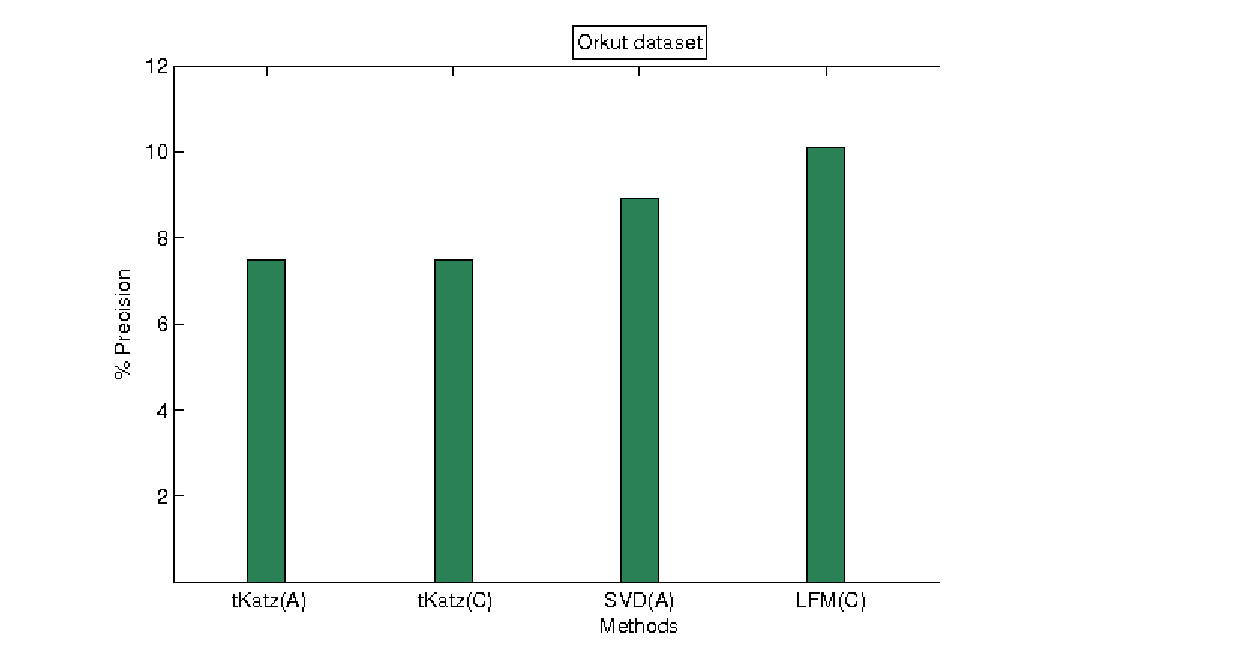
\includegraphics[scale=0.35]{OrkutLinkPredictionEvaluation.eps}}
    \subfigure[Youtube data set]{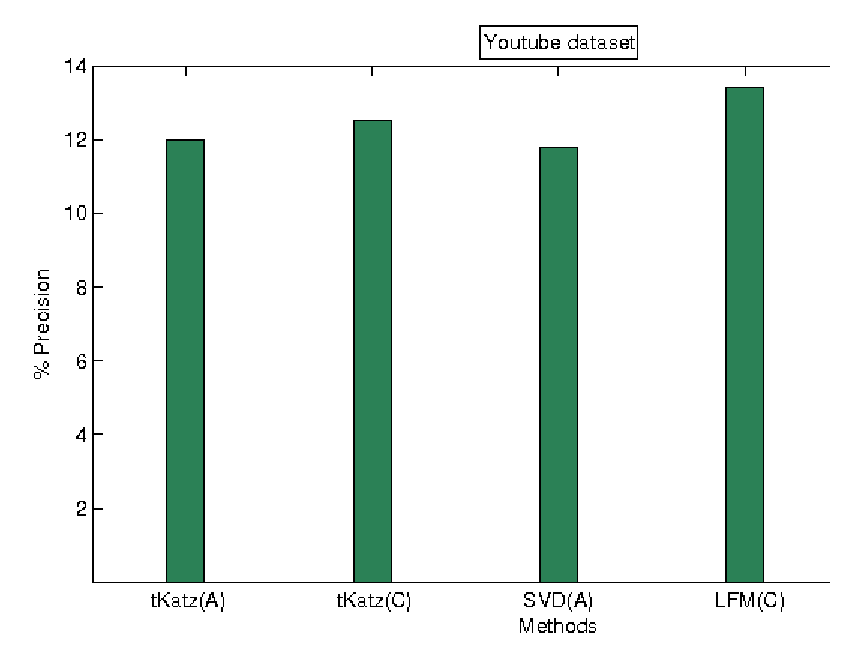
\includegraphics[scale=0.35]{YoutubeLinkPredictionEvaluation.eps}}
  \end{center}
  \caption{In this figure, various recommendation algorithms are compared using the ``global'' sensitivity measure described in Section \ref{sec:globalVsPerUserEvaluationMethods}, where a total of $\sum_u E_u$ recommendations are made, with no guarantees about the number of recommendations made for any given user. According to this evaluation method, LFM($\C$) appears to be superior to \textsf{tKatz}($\C$). However, these results are different from those described in Figure \ref{fig:summaryResults}, where recommendation algorithms are compared based on the goodness of the top 50 recommendations made for the average user.}
  \label{fig:linkPredictionEvaluation}
\end{figure}

\begin{figure}[ht]
  \begin{center}
    \subfigure[Orkut data set]{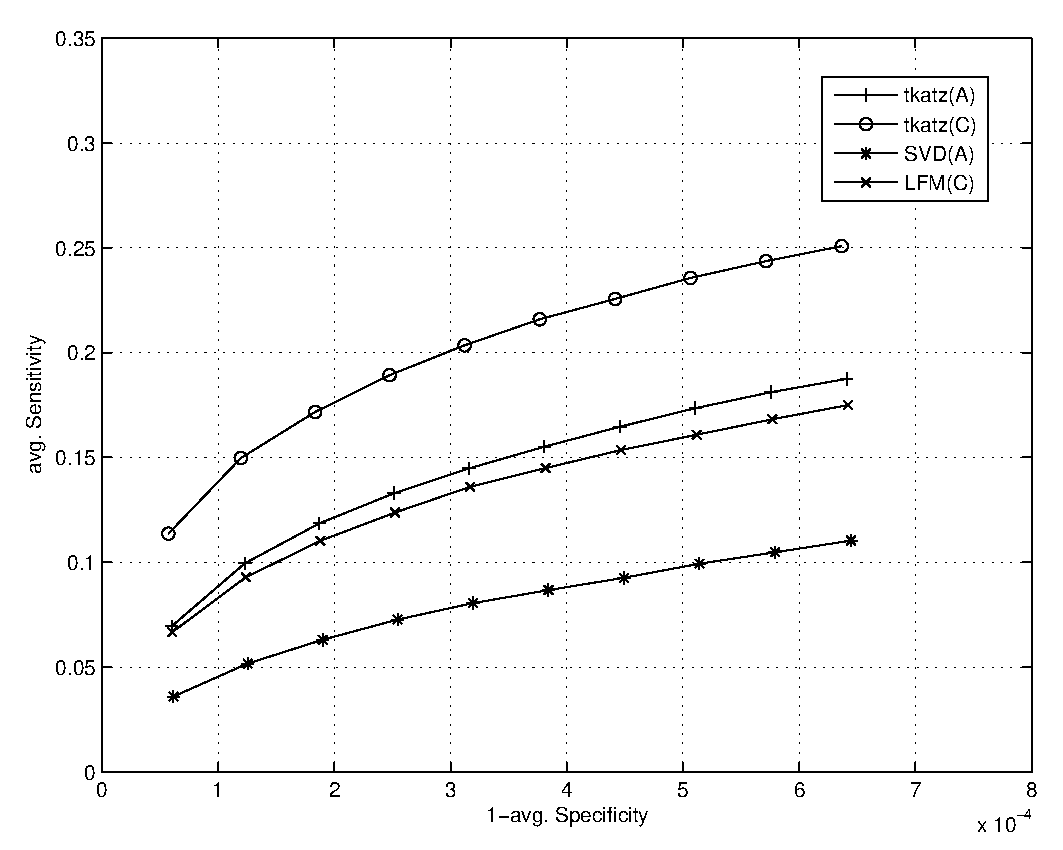
\includegraphics[scale=0.35]{summaryOrkut.eps} \label{fig:sumRes-a}}
    \subfigure[Youtube data set]{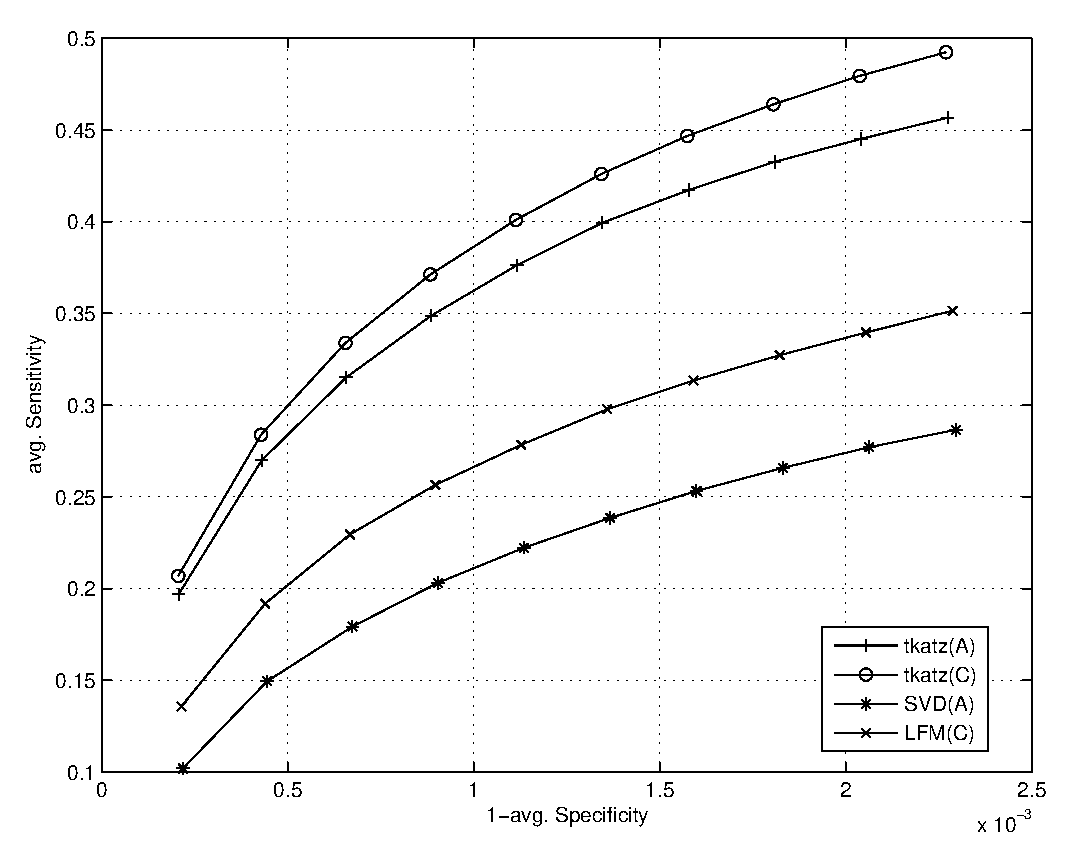
\includegraphics[scale=0.35]{summaryYoutube.eps}\label{fig:sumRes-b}}
  \end{center}
  \caption{Comparison of recommendation algorithms based on graph proximity and latent factors models, as described in Section \ref{Evaluation method}. The leading portion of the ROC curve is shown, thus recommendation algorithms are compared based on the goodness of their top 50 recommendations. The graph proximity based predictors consistently outperform latent factors based predictors in the two data sets. See Section \ref{Results and Discussion} for further discussion.}
  \label{fig:summaryResults}
\end{figure}

\begin{figure}[ht]
  \begin{center}
    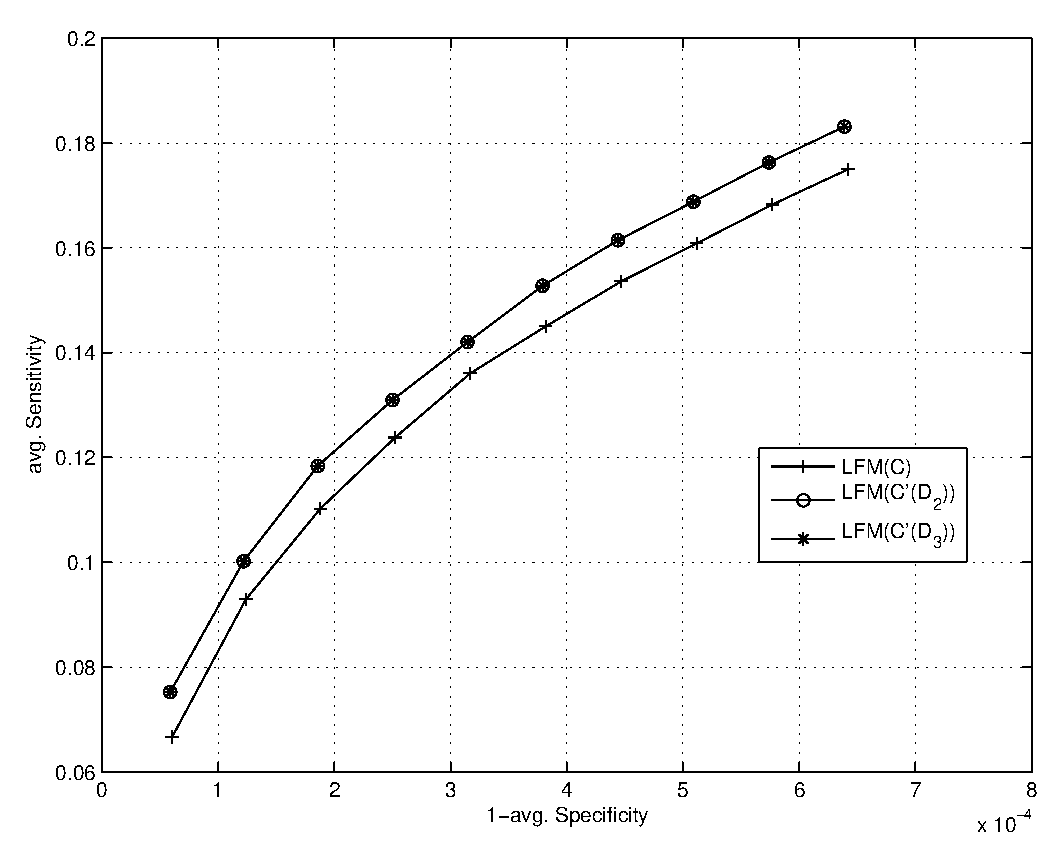
\includegraphics[scale=0.66]{summarySVDOrkut.eps}
  \end{center}
  \caption{Comparison of latent factors based algorithms for various choices of $\D$, for the Orkut data set: $\D_{2} = \A^{T}\A, \D_{3} = \lambda \A^{T}\A$.}
  \label{fig:summarySVD}
\end{figure}


\subsection{Results and Discussion}
\label{Results and Discussion}
\begin{table}[h!]
\centering
\begin{tabular}{| c | l |} \hline
\textsc{Experiment}&\textsc{Score Matrix}\\ \hline
\textsf{tKatz}(\A) & \textsf{tKatz}$(\A\A^T, \beta, k) \A$ \\ \hline
\textsf{tKatz}(\C) & Equation (\ref{e:tKatzC}) \\ \hline
SVD(\A) & SVD(\A) \\ \hline
LFM(\C) & Equation (\ref{e:LFM}) \\ \hline
LFM-c(\C, $c$) & Equation (\ref{e:clustLowRankC}) extended to $c$ clusters\\ \hline
\textsf{tKatzCS}($d$) & Equation (\ref{e:tKatzCS}) \\ \hline
\textsf{tKatzLFM}(\C, $d$) & \textsf{tKatz}($\C_d$), where $\C_d$ is rank-$d$ approximation of \C \\ \hline
\textsf{tKatzLFM-c}(\C, $c$, $d$)) & \textsf{tKatz}($\C_d$), where $\C_d$ is the clustered rank-$d$ approximation of \C \\ \hline
\end{tabular}
\caption{List of experiments, with the score matrix used for ranking the user-group connections, based on latent factor and graph proximity models.}
\label{tab:experiments}
\end{table}

In this section, we report and analyse the performance of the various recommendation algorithms, based on the graph proximity model and latent factors model discussed in Sections \ref{Models} and \ref{Scalability}. We compare the performance of the graph proximity methods with the latent factors methods on the average sensitivity and average specificity metrics introduced earlier, for a given number of recommendations in $\{ 5,10,\cdots,45, 50\}$.  We study the performance of the scalable approximation methods proposed in Section \ref{Scalability}, and compare these methods amongst themselves and with the methods proposed in Section \ref{Models}. The list of experiments based on latent factor and graph proximity predictors are presented in Table \ref{tab:experiments}.

\subsubsection{Performance of recommenders based on the two models}
Consider the performance of the recommendation algorithms on the Orkut data set in Figure \ref{fig:sumRes-a}. SVD($\A$) gives the lowest performance of all the methods. LFM($\C$) performs better than SVD($\A$), which is expected given that it uses information from the friendship network $\SS$ in addition to the information from affiliation network $\A$. For the average user, the graph proximity model based methods significantly outperform latent factors based methods as observed in both plots of Figure \ref{fig:summaryResults}. In particular, we see that \textsf{tKatz}($\C$) performs much better than \textsf{tKatz}($\A$), which in turn outperforms latent factor based methods. We see that the information in the friendship network indeed proves highly beneficial in making affiliation recommendations and graph proximity based methods exploit this information the most. A summary of performances of the algorithms on the Youtube data set are shown in Figure \ref{fig:summaryResults} (b). We observe that the case for Youtube is similar to that of Orkut, in that graph proximity based algorithms significantly outperform latent factors based algorithms. In particular, \textsf{tKatz}($\C$) is highly successful compared to the other methods. 


Another interesting comparison of latent factor methods based on the choice of $\D$ in constructing the combined network $\C'$ given in (\ref{e:generalizedCombined}), is presented in Figure \ref{fig:summarySVD}. We observe that the choice of $\D$ does not appear to make any significant difference in the performance of the recommendation algorithm. In the plot we use $\D_2 = \A^{T}\A$ and $\D_3 = \lambda \A^{T}\A$, where $\lambda$ is also the weight associated with $\SS$ in the combined graph. Even though, in case of the Orkut data set, we see that SVD($\C', \D$) performs slightly better than SVD($\C$), it appears as if scaling $\D \neq 0$ does not affect recommendation quality. In case of Youtube (plots not shown), our experiments indicate that $\D$ is not useful at all. The obvious choices for $\D$ do not seam to improve the performance compared with $\D = 0$.


The best parameters learned by the various algorithms are presented in Table~\ref{tab:parameters}. Note that the best parameter $\beta = 10^{-12}$ implies that the calculated \textsf{tKatz} measure was effectively using the common neighbors method. In other words, users and communities connected by path lengths 5 or more\footnote{Corresponding to 2nd and higher powers of $\beta \A\A^{T}$ in \textsf{tKatz}(\A).} are not useful in making affiliation recommendations.

\begin{table}[t!]
\centering
\begin{tabular}{| c | p{2.4cm} | p{2.4cm} |} \hline
Algorithm&Orkut&Youtube\\ \hline
LFM($\C$) & $d=50, \gl = 0.8$ & $d = 90, \gl = 1$ \\ \hline
LFM($\C'(\lambda \A^{T} \A)$) & $d = 60, \gl = 0.6$ & $d = 70, \gl = 1$ \\ \hline
\textsf{tKatz}($\A$) & $\gb = 10^{-12}$ & $\gb = 10^{-12}$ \\ \hline
\textsf{tKatz}($\C$) & $\gb = 0.01, \gl = 0.2$ & $\gb = 0.1, \gl = 0.4$ \\ \hline
\end{tabular}
\caption{Best parameters learned by the recommendation algorithms using validation.}
\label{tab:parameters}
\end{table}

We see that the recommendation algorithms perform consistently across the two data sets, and the evaluations are robust as the specificities and sensitivities are averaged over 9000 users in Orkut and 16000 users in Youtube.

\subsubsection{Scalable approximations to \textsf{tKatz}(C)}
From Figure \ref{fig:summarySVDKatz}, we observe that in general, combining ideas from the latent factor model with graph proximity model yields better performance than simply using the low rank approximations of $\C$. The exception to this is the case of recommendations made by LMF-c on the Orkut-1c data set, here \textsf{tKatzLMF-c} decreases the quality of the predictions made by LMF-c further.

In Figure \ref{fig:summaryScalability}, we observe that the recommendation quality of the scalable recommenders proposed in this paper is close to that of \textsf{tKatz}($\C$). In particular, we note that \textsf{tKatzCS} consistently performs very well on both data sets. Comparing the performance of \textsf{tKatzLFM} and \textsf{tKatzLFM-c}, we also note that the use of clustering is effective in improving performance, and this suggests that we can perhaps derive similar benefit out of considering a clustered version of the \textsf{tKatzCS} algorithm.

Finally, in Figure \ref{fig:summaryDependency}, we study the effects of change in the number of clusters and the number of factors used on the performance of algorithms which use graph clustering for the purpose of scalability. We observe that changing the number of clusters does not make a significant difference in performance, whereas increasing the number of factors yields better performance. This is not surprising considering the fact that these algorithms can be viewed as computing approximations of \textsf{tKatz}($\C$).

\begin{figure}[ht]
  \begin{center}
    \subfigure[Orkut-1c data set]{\includegraphics[scale=0.35]{summarySVDKatzOrkut.eps}}
    \subfigure[Youtube-1c data set]{\includegraphics[scale=0.35]{summarySVDKatzYoutube.eps}}
  \end{center}
  \caption{In this figure, we observe that, in general, combining ideas from the latent factor model with ideas from the graph proximity model yields better performance than simply using the low rank approximations of $\C$ in isolation. This is consistent with our observations in Figure \ref{fig:summaryResults}. See Section \ref{Results and Discussion} for further discussion.}
  \label{fig:summarySVDKatz}
\end{figure}

\begin{figure}[ht]
  \begin{center}
    \subfigure[Orkut-1c data set]{\includegraphics[scale=0.35]{summaryScalabilityOrkut.eps}}
    \subfigure[Youtube-1c data set]{\includegraphics[scale=0.35]{summaryScalabilityYoutube.eps}}
  \end{center}
  \caption{Comparison of the performance of the proposed scalable graph proximity based methods. In this figure, we observe that the recommendation-quality of the scalable recommenders proposed in this paper is close to that of \textsf{tKatz}($\C$). In particular, we note that \textsf{tKatzCS} consistently performs very well on both data sets. Comparing the performance of \textsf{tKatzLFM} and \textsf{tKatzLFM-c}, we also note that the use of clustering is effective in improving performance.}
  \label{fig:summaryScalability}
\end{figure}


\begin{figure}[ht]
  \begin{center}
    \subfigure[Effect of changing the number of clusters.]{\includegraphics[scale=0.35]{summaryClusteredMethodsClusterDependencyYoutube.eps}}
    \subfigure[Effect of changing the number of factors.]{\includegraphics[scale=0.35]{summaryRankDependencyYoutube.eps}}
  \end{center}
  \caption{In this figure, we study the effects of change in the number of clusters and the number of factors used on the performance of algorithms which use graph clustering for the purpose of scalability. These experiments were conducted on the Youtube-1c data set. We observe that changing the number of clusters does not make a significant difference in performance, whereas increasing the number of factors yields better performance. This is not surprising considering the fact that these algorithms can be viewed as computing approximations of \textsf{tKatz}($\C$).}
  \label{fig:summaryDependency}
\end{figure}


%\begin{table}[ht]
%\centering
%\begin{tabular}{| c | p{2.4cm} | p{2.4cm} |} \hline
%Algorithm& Runtime\\ \hline
%SVD($\C$)& 71.4\\ \hline
%SVDcl($\C$, 5) & 191.1\\ \hline
%tKatz($\A$)& 27.3\\ \hline
%tKatz($\C$)& 96.2\\ \hline
%tKatz(SVD($\C$))& 90.3\\ \hline
%tKatz(SVD($\A$, 300), SVD($\SS$, 300))& 1160\\ \hline
%tKatz(SVDCl($\C$, 300))& 644\\ \hline
%\end{tabular}
%\caption{Run-times in seconds of various algorithms on a 2.5GHz machine with 512KB cache.}
%\label{tab:runTimes}
%\end{table}




\section{Conclusion and Future Work}
\label{Conclusion and Future Work}
In this paper, we have tackled the affiliation recommendation problem, where the task is to recommend new affiliations to a given user, given the current state of the friendship and affiliation networks. We show that information from the friendship network can indeed be fruitfully exploited in making affiliation recommendations. This auxiliary source of information was hitherto not used in making community recommendations.

Using a simple way of combining these networks, we suggested two ways of modeling the networks for the purpose of making affiliation recommendations (Section \ref{Models}). The first of these approached the problem from the graph proximity viewpoint, whereas the second modelled the interactions of users and groups in the two networks using latent factors derived from optimizing towards a joint matrix factorization objective. We studied the algorithms suggested by these models on real world networks (Section \ref{Experimental Evaluation}). We motivated and proposed a way of evaluating recommenders, by measuring how good the top 50 recommendations are, and demonstrated the importance of choosing the right evaluation strategy. Algorithms suggested by the graph proximity model turn out to be the most effective, based on experiments on large real world data-sets. These results show that the application of techniques from social network link prediction in affiliation and item recommendation is a promising one.

\subsection{Future Work}
There is the intriguing possibility of using an affiliation network for link prediction in the friendship network. Discovering techniques and models which do this effectively seems to be a challenging research avenue. Our early experiments at doing this indicate that this is a much harder problem. The reasons for this are not yet clear, and this question seems fertile for further exploration.

Within the ambit of the affiliation recommendation problem itself, one may research the ways of fruitfully using even more sources of information. For example, Chen et al\cite{GoogleCCF} use information from textual description of communities along with the affiliation network to make affiliation recommendations. It might be useful to consider the social network together with this auxiliary information. Also, predictors based on latent factors model and the graph proximity model may be suited for different types of users, and creating a meta-predictor which combines predictions from both classes of predictors is another attractive research direction. Scalability is a challenge in using predictors based on the graph proximity models on massive datasets - both in terms of memory and in terms of computational cost\cite{savas10c}, and developing efficient predictors based on the graph proximity model will be part of future work.


\section{Acknowledgements}
We thank Prateek Jain for helpful discussions. Zhengdong Lu is supported by an ICES postdoctoral fellowship at UT Austin. 
Berkant Savas is supported by the Swedish Research Foundation international postdoctoral fellowship and ICES.
This research was supported by NSF grants CCF-0916309 and IIS-0713142.

\bibliographystyle{acmtrans}
\bibliography{../paper/references,myBibsEN}

\end{document}
